\documentclass[a4paper, 10pt, conference]{report}
\usepackage{titlesec}
\usepackage{enumitem}
\usepackage{hyperref}
\usepackage{graphicx}
\usepackage{rotating}
\usepackage{float}
\usepackage{units}
\usepackage{pifont}
\usepackage{enumitem}
\usepackage{qtree}
\usepackage[export]{adjustbox}
\usepackage[numbers,sort]{natbib}
\usepackage{listings}
\titleformat{\chapter}{\normalfont\huge}{\thechapter.}{20pt}{\huge\textbf}
\newcommand{\cmark}{\ding{51}}%
\newcommand{\xmark}{\ding{53}}%
\newcommand{\nospace}{\setlength\itemsep{0em}}
\begin{document}
\author{J.J. Schutte, University of Twente\\\emph{j.j.schutte@student.utwente.nl}}
\date{June 27, 2019 \\ \vspace{26em} 
\includegraphics[width=\textwidth ,center]{resources/img/logos.png}}
\title{\textbf{Master Thesis} \\Design of a development platform to monitor and manage Low Power, Wide Area WSNs
}
\maketitle
%\begin{titlepage}
%\large
%\centering
%{\Huge{Master Thesis}\\}
%{\Large{Design of a development platform to monitor and manage Low Power, Wide Area WSNs}} \\

%J.J. Schutte, University of Twente \\
%\emph{j.j.schutte@student.utwente.nl} \\
%June 27, 2019
%\end{titlepage}


\abstract{The recent explosion of Low Power Wide Area (LPWA) WSN devices has raised interest in perceiving the Quality of Service (QoS) provided to and by such applications. Current QoS solutions do not respect LPWA-specific considerations, such as limited resources and extreme scale. This study has set out to research an appropriate solution to QoS monitoring and management that does concern these considerations. This is achieved by establishing a development platform focused on LPWA QoS. The platform consists of two chief concepts. The first of which is a distributed stream processing architecture. The architecture back-bone is based on Apache Storm and provides scaffolding for different classes of stream transformations, which guides users in implementing their monitoring applications. The second artefact is a model capable of captivating resources and calculating the performance of a system, considering different modes of operation of that system. The proposed development platform is validated by implementing an instantiation of it, based on an actual, commercial on-street parking application. Though the study shows some deficiencies still present in the solution, its results demonstrate it as an applicable and feasible aid in constructing scalable applications capable of QoS monitoring in LPWA WSNs. \\ \\
%{Keywords --- WSN, IoT, LPWA, QoS}
\textbf{Keywords}: Wireless Sensor Networks, Internet of Things, LPWA, Quality of Service
\subsubsection*{Committee}
This thesis was supervised and examined by:
\begin{table}[h]
\begin{tabular}{ll}
prof.dr.ir. M. Aksit & University of Twente, Formal Methods and Tools \\
dr. N. Meratnia & University of Twente, Pervasive Systems\\
R. Boland & Nedap N.V., Identification Systems \\
\end{tabular}
\end{table}
%\item[prof.dr.ir. M. Aksit] Formal Methods and Tools - University of Twente
%\item[dr. N. Meratnia] Pervasive Systems - University of Twente
%\item[R. Boland] Nedap N.V.
\newpage
\tableofcontents
\newpage
\chapter{Introduction}

\section{Domain overview} 
Wireless Sensor Networks (WSNs) have received large amounts of research the past decades. However, this mainly resulted in isolated ad hoc networks. With both the size of WSN's and the amount of networks increasing, the deployment of multiple networks in the same geographical area for different applications seemed increasingly illogical. Therefore, recent endeavours have attempted design networks and protocols in order to create a general, ubiquitous internet for automated devices and sensors: the Internet of Things (IoT). A specific recent development in IoT has focussed on the field of Low Power Wide Area networks (LPWA). These networks serve devices that communicate over large distances with very limited computational and communication resources \cite{value_of}. They therefore entail low data rates, low radio frequencies and raw unprocessed data

These extremely restrictive requirements entail that a regular wireless internet connection does not suffice, as it is not optimized for the extreme resource limitations of LPWA IoT applications. Multiple corporations are developing and deploying exclusive wide area networks for low powered devices. Examples of these networks are Narrow-Band IoT \cite{nbiot}, LoRaWAN \cite{web:lora} and Sigfox \cite{web:sigfox}. These networks are deployed and operated by telecom providers and allow instant connectivity by incorporating a SIM or proprietary network connectivity module. As a consequence large-scale LPWA applications are moving from node-hopping and mesh network strategies to operated cell networks \cite{movement_to_cellular, movement_to_cellular_2}. Because of the aforementioned reasons the number of connected devices has exploded in the recent years. Estimations vary but a consensus established from multiple sources predict about 15-30 billion connected devices in 2020 \cite{nr_devices_gartner, nr_devices_forbes, security_risks_ocean_connect, nr_devices_ericsson}. This would imply that by 2020 the number of connected IoT devices will have surpassed the number of consumer electronic devices (e.g. PC's, laptops and phones) \cite{nr_devices_ericsson}.

Both the explosion of devices, entailing explosion of data, and the shift to shared operated cell networks implies a great stress on monitoring sensor applications. While relatively small sized applications on proprietary networks allow for a best-effort approach, the convolution of many large applications on a shared network requires knowledge of the performance provided by the application. The term coined for this is Quality of Service (QoS). QoS parameters such as application throughput, service availability and message drop allow the description of the performance state of a system or application \cite{qos_definition}. It is therefore paramount for a commercial application to have its QoS metrics observed.

The notion of QoS in a networked application is not a novel concept. It has been a research and industry paradigm for as long as commercial applications have existed. Consequently, many forms of QoS monitoring and management exist for regular internet and networking applications. However, these methods do not transfer well to the field of WSN and IoT, as will become apparent in this section. This presents a vacancy that requires exploration. Access to such QoS solutions will improve the maturity and operational feasibility of commercial, large-scale IoT applications.

The remainder of this introductory chapter will determine some of the key challenges which differentiate QoS monitoring of regular networks and wireless sensor networks. The next section will deliberate some key obstacles in the current state of art of monitoring Quality of Service in LPWA Wireless Sensor Networks. Subsequently, it will be deliberated why existing solutions cannot provide for the QoS monitoring  needs of LPWA applications. After which the succeeding section will introduce the proposed approach to design a development platform for applications to deal with these challenges and capture the QoS in WSN's.
%TODO WSN & IoT interchangeble


\section{Challenges in monitoring QoS in LPWA}
\label{sec:challenges}
Three key challenges were identified that fundamentally complicate QoS measurement and management in LPWA networks and applications. These challenges affect the applicability of conventional QoS mechanisms to the field of IoT and WSN. %These causes will be shortly deliberated individually before summarizing the implications they effect on the domain of QoS monitoring.

\subsubsection{Technical limitations of end-devices}
The first challenge of LPWA applications are the previously mentioned extreme resource constraints \cite{key_features, value_of}. For example, LPWA devices are expected to communicate on a network shared by a vast amount of nodes, diminishing the individual connectivity resources. As a consequence, uplink communication is regularly aggregated over time and transmitted opportunistically. Therefore, back-end applications are required to facilitate irregular and infrequent reporting intervals from sensor nodes. Additionally, an LPWA device is required to perform for a certain amount of time, typically at least 10 years \cite{tmobile, vodafone, nbiot_vs_lora}, on a finite battery energy supply. Therefore, there are no resources to spare for expensive auxiliary processes \cite{energy_challenges}. Consequently, devices usually send low-level auxiliary data, instead of intelligently derived values. The burden of calculating high level information is then deferred to be computed in-network (edge computing) or at the back-end application server.

Additionally, evolution of sensor device software is far more restrictive then evolution of back-end application's software. Firstly, because of the long life-time of devices, it can occur that services based on modern day requirements need to be performed by decade old technology. Secondly, most LPWA networking protocols do not require devices to retain a constant connection in order to save energy (duty cycling) \cite{tmobile, vodafone, on_duty_cycling, energy_challenges}. Instead, the devices connect periodically or when an event/interrupt occurs. This entails that devices are not updated \emph{en masse}, but individually when a device wakes up. As this requires additional resends of the updated code it consumes more connectivity resources in the network. 

For these reasons LPWA sensor applications often employ a \emph{"dumb sensor, smart back-end"} philosophy. Consequently, the computations are deferred to the network, back-end or cloud \cite{popularity_applications_qos_moeilijk, defer_cloud}. The problem however with deferring the computations further to the back-end is that more and more computations have to be performed centralized. This requires the back-end to be extremely scalable because more tasks need to be performed as more devices are added to the application \cite{stream_requirements, iot_big_data_difficulties, qos_tradeoff}.

\subsubsection{IoT QoS is different}
Aside from the low-level information sent by the large amount of devices, QoS in WSNs is distinctly different from classical client-server QoS. Often QoS in a client-server application can be measured at the server. QoS monitoring in a cloud environment may require some aggregation of data, but even then the number of data sources is relatively limited. Large WSN applications require data aggregation by default. As the Quality of Service provided by the application can only be ascertained by calculations based on auxiliary data collected from a huge number of devices. This concept is known as Collective QoS \cite{qos_specific_wsn} and comprises parameters such as collective bandwidth, average throughput and the number of devices requiring replacement. As this information eventually requires accumulation on a single machine in order to determine concrete values, aggregation of expansive volumes of auxiliary sensor data must be performed intelligently as not to form a congestion point or single point of failure.

However, device level information is still required alongside of collective QoS \cite{device_level}. If a device is not performing according to expectations of a predetermined strategy, it is required that this is mitigated or informed. This introduces a second distinction to classical QoS: multi-level monitoring and reporting. Conventionally, only the QoS provided by the server(s) running an application is of interest. However, in a wireless sensor environment, monitoring of parameters on different levels is required. Examples of these monitoring levels are single sensor, the application as a whole or analysis per IoT cell tower or geographic area. This requirement entails data points of different levels of enrichment, calculated from the same raw sensor data.

The final distinction in IoT monitoring is the dynamic nature of WSN applications \cite{popularity_applications_qos_moeilijk}. Firstly, an IoT monitoring application needs to be prepared for devices added to the network and dropping out of the application \cite{ontology}. As a collective QoS parameter is based on a selection of devices, the monitoring application must support adding and remove devices from the equation. Additionally, diverse deployment of nodes causes them to behave differently. Therefore, QoS procedures should account for the heterogeneity exhibited throughout the WSN \cite{energy_challenges}.

In conclusion, IoT QoS management will require a flexible and dynamic method of resource parameter modelling. Additionally, this process should be able to be applied to a high influx of sensor date. This monitoring technique should be able to calculate both lower level (single sensor) and higher level (application) resource distribution.

\subsubsection{Movement to operated cell network}
A final challenge in contemporary QoS monitoring of LPWA applications is the earlier recognised increasing trend of shared, telecom-operated cell networks \cite{tmobile, vodafone}. Though it makes IoT connectivity more efficient because many applications can be served by a single network infrastructure, it  effects complications to the QoS. Firstly, Many applications will be competing for a shared scarce amount of network resources. When other applications consume a large portion of the resources, due to poor rationing or event-bursts, your application suffers and cannot provide the expected QoS.

Secondly, by out-sourcing the network infrastructure, control over the network is lost. Though beneficiary to the required effort, some important capabilities are conceded. For example the network can no longer be easily altered in order to suit the needs of the application. Additionally, auxiliary data can not be extracted from the network and edge computing is not an option, again deferring the burden of aggregating QoS data entirely to the back-end.

Finally, the telecom operator will require adherence to a Service Level Agreement (SLA). Though this ensures a certain service provided to an application and prevents other applications of consuming extraneous resources, it also requires close monitoring of applications. A breach of the SLA may cause fines or dissolving of a contract. Therefore, strict adherence to the SLA parameters is necessary and timely proactive intervention is required, if the limits of the SLA are threatened to be exceeded \cite{cloud_computing_monitoring}.

To summarize, outsourcing the management of the network infrastructure to a professional telecom provider aggravates the need for exact and real-time curtailment of digital resources, while simultaneously impeding the ability to do so in the network itself. This will need to be remedied by adapting the parts of the WSN architecture within the domain of control, i.e. the sensor devices and the back-end application. Because of the earlier proposed concerns and challenges this increased responsibility will be mostly attributed to the back-end application.

%\subsubsection{Summary}
%In conclusion, The tendency to defer computations challenges the computing capabilities of centralized solutions. This inability for pre-computation, combined with immense input numbers of LPWA device data, entails a design with a deliberate focus on scalability of throughput. Additionally measuring and controlling QoS in Wireless Sensor networks is very different from measuring and controlling QoS in resource-abundant networks. Both because of the resource constraints and the fact that the QoS characteristics in WSN's are different from the characteristics in conventional networks and applications. Finally, by outsourcing the responsibility of network management, the ability to control and observe those networks is also lost.

%To this purpose we will research the applicability and design of a WSN QoS platform. This platform should address the issues of scalability and limitations of source devices and in-network processing. It should be noted however that we will not address the issues of end-device resource restriction and network obscuration directly, only the challenges it imposes on the task of QoS monitoring and control.

\section{Current State of the Art}
The previous section illustrated some key challenges in measuring and determining QoS in WSNs. This section will deliberate on some known QoS protocols and existing monitoring solutions. It will conclude by arguing why the current state of the art does not provide a suitable solution for the previously identified challenges.

\subsection{QoS protocols}
\label{sec:qos-protocols}
The first well known protocol often employed for QoS monitoring is SNMP \cite{snmp}. SNMP provides a formalized, device-independent addressing scheme to request key device and networking data points. Additionally, it allows application developers to specify custom addressable data points. Though SNMP does not feature command and control capabilities, the information obtained by it can be used to configure and control an application by other means.

A protocol that does feature such command \& control capabilities is Integrated Services (IntServ) \cite{intserv_diffserv_uitleg}. This protocol negotiates a resource allocation in the network per data flow. This allocation is then permeated throughout the network domain and retained until the data flow has ended. It provides hard QoS guarantees within the network, but at a severe preparation cost and overhead.

A more cost-efficient QoS protocol is Differentiated Services (DiffServ) \cite{intserv_diffserv_uitleg}. This protocol does not require resource negotiation and instead identifies differentiating traffic classes. Depending on the determined class, the data will enjoy specific benefits such as priority handling or increased network resources allocation. Though the QoS guarantees provided by this protocol are softer than that of IntServ, it also generates vastly less overhead.

The former protocols are all general application networking protocols. Though there are proposals for IoT-specific QoS monitoring frameworks. A promising solution is presented by R. Duan et al \cite{qos_extensive_architecture}. This framework aims for an automated negotiation procedure between node, network and back-end layers in order to deliberate a reporting level that compromises the monitoring needs with the available resources and device capabilities. In this manner it can offer the greatest benefit to QoS without considerably impacting it negatively.

\subsection{QoS platforms}
Aside from protocols managing QoS there also exist some IoT platforms that are capable of (or enable) some form of QoS monitoring. This section will detail three of them and how they curtail the posed challenges or are invalidated by them.
\subsubsection*{PTC ThingWorx}
PTC ThingWorx \cite{web:thingworx} is a proprietary IoT PaaS solution developed by PTC. It is a full-scale cloud platform offering many prepackaged IoT support services. The focus of this platform is on rapid application design, development and deployment. The aim of the ThingWorx team is to offer the ability to develop IoT applications without coding and instead device an application by only using the ThingWorx application interface. This simplifies the development cycle and shortens time-to-market \cite{study_of_various}. Though it is capable of monitoring the performance of an application, the focus of the platform is on application development and data management. Therefore, employing it for performance monitoring only might be a disproportionate approach, especially considering that ThingWorx is a paid platform. Additionally, only using a small section of the platform's functions might lead to installing bulky, cumbersome agents in sensor devices. This will potentially unnecessarily consume resources of a constraint device. Aside from the previously mentioned extravagances, sources report that ThingWorx has scalability problems \cite{good_assessment}.% and difficulties with technical expertise and communication in their professional services devision \cite{forrester}.

\subsubsection*{Cisco Jasper Control Center}
Cisco has extended its Jasper cloud platform and has optimized it for several IoT markets. This extension includes a product specifically designed for LPWA IoT applications named the Control Center for NB-IoT \cite{cisco_jasper}. It is specifically designed for SIM-connected (LTE) device connectivity management \cite{forrester}. It accomplishes this through Cisco's proprietary network hardware and partnerships with mobile operators that incorporate data extraction end-points in their devices. Jasper therefore focuses on data and information obtained from network nodes and edge computation instead of communicating with actual end-devices. This decreases the burden on resource constraint devices and alleviates the challenge posed by the movement to provider operated cell networks. However, in doing so it neglects information that can only be acquired by node inspection

Jasper Control Center allows the usage of business rules for information extraction and actuation, and can employ outbound communication channels (e.g. email or SMS) for alerting purposes.  In addition it includes API's for more complex further analyses. Jasper Control Center is a proprietary SaaS solution which can be procured in packages. However, the basic packages seems to only include minimal functionality and more advanced functions such as rule-based automation and third party API access are sold in separate additional packages \cite{cisco_jasper}. Finally, Jasper Control Center can report on a few Collective QoS parameters (e.g. data usage, number of reports received), but it has been reported that Jasper lacks in analytic functionality \cite{forrester}.

\subsubsection*{Nimbits}
Nimbits \cite{web:nimbits} is an open-source cloud data logger and analysis PaaS. It employs a rule-based engine to filter, log and process incoming data. Additionally, rules can be defined to instruct the engine to report alerts via external communication channels. It operates by defining data points to which sensors and servers can write and read data \cite{study_of_various, nimbits_mqtt}. Devices can do so by employing a Nimbits client or via HTTP API's. It has been reported that Nimbits can communicate via the light-weight MQTT protocol \cite{nimbits_mqtt}, but documentation demonstrating this is lacking. It therefore appears that Nimbits lacks the considerations required for resource constraint LPWA devices.

Nimbits is not primarily intended as a QoS monitoring platform, but can be configured as such by regarding auxiliary QoS data as primary data of a dedicated QoS monitoring application. However, after analysing Nimbits's design of data points, Nimbits seems to be most appropriate for applications with a small pool of distinct sensor types. Establishing and managing data points for a colossal amount of devices of equivalent data types, as a monitoring job will often encompass, rapidly becomes a cumbersome effort to automate.

%TODO zoveel mogelijk referenties naar challenges
\subsection{Deficiencies in current state of art}
\subsubsection{QoS protocols}
The protocols described in Section \ref{sec:qos-protocols} are unfortunately not applicable to the LPWA WSN domain. Firstly, SNMP generally operates according to a master-slave architecture \cite{snmp_server_initiated} which requires slaves (sensor nodes) to remain on-line permanently, or at least regularly \cite{snmp_architecture}. This demand is invalidated by the resource restriction complication featured in LPWA applications \cite{key_features}. This can be partly alleviated by proxying the sensor devices by a proxy that is less resource constrained. This would however come at the cost of a lack of real-time data or delayed response times \cite{snmp_proxy}. Therefore, a more appropriate solution would be to employ a client-initiated approach. Furthermore, SNMP and related protocols consider end-to-end QoS. As discussed in Section \ref{sec:challenges}, WSN application monitoring must consider both end-to-end and Collective QoS. Therefore, even if SNMP is employed, further processing is required.

Though IntServ's hard QoS guarantees are powerful, the overhead required to establish these flows is far too imposing \cite{intserv_diffserv_too_complex, qos_challenges}. Since LPWA only sends small message payloads, the heavy per flow negotiation data will easily exceed the payload data. With LPWA's limited resources in mind this cannot be considered as an efficient solution. Conversely, DiffServ does not feature this immense overhead cost. However, application of the protocol is complicated by the movement to commercial network operators, as it would require them to implement a class-based allocation system in their networks. The previously mentioned inhibitions are potentially aggravated by local net neutrality laws. Though this was not a concern in privately operated proprietary networks, in universal Internet of Things extreme networks severe net neutrality laws may prohibit priority treatment of data flows based on their source, destination or content \cite{net_neutrality}. This implies that the required QoS guarantees cannot feasibly or legally be (fully) provided by a commercial Internet of Things network provider and in-network protocols
%TODO citesdiffserv

Furthermore, both IntServ and DiffServ consider only network QoS, therefore they lack the level of inspection to report or consider the state of limited resources in end-devices. This deficiency also troubles IoT-specific QoS protocols. Most efforts are focussed towards efficient and effective networking in order to facilitate increasing data-rates. These protocols disregard important device metrics, such as node lifetime and sensor measurement accuracy, which are paramount to determining the health and performance of an IoT application. Finally, though the protocol of R. Duan et al \cite{qos_extensive_architecture} does feature this level of inspection, the details require further implementation to fully complete the protocol. Since the field of IoT is relatively young, no such IoT-specific QoS procedures have matured to a uniform and universal internet standard. From the preceding it is concluded that contemporary general purpose or IoT-specific QoS protocols cannot provide for an adequate in-network solution. Instead, this obligation is imposed on the back-end and the end-devices.

%TODO check footnote is on page
%TODO plaatsing
\subsubsection{QoS platforms}
\begin{table*}[t]
\begin{minipage}{\textwidth}
\centering
\begin{tabular}{|l|c|c|c|c|c|} \hline
 & ThingWorx & Cisco Jasper & Nimbits \\ 
 & & Control Center & \\ \hline
LPWA specific\footnotemark & \xmark & \cmark &  \xmark \\ \hline
QoS monitoring focus & \xmark & \xmark & \xmark \\ \hline
Open-source & \xmark & \xmark & \cmark \\ \hline
Device-level inspection & \cmark & \xmark & \cmark \\ \hline
Extreme scalability & \xmark & \cmark & \xmark \\ \hline
\end{tabular}
\caption{Comparative analysis of IoT QoS monitoring platforms}
\end{minipage}
\label{table:platform_assessment}
\end{table*}

\footnotetext{I.e. constrained by resource limitations}

An assessment of the discussed platforms and their applicability to the field of LPWA is depicted in table \ref{table:platform_assessment}. It shows that these platforms are all lacking in some important considerations. These platforms are either not conceived with a focus on LPWA's severe resource constraints, a primary focus on resource and QoS monitoring or the extreme scale of contemporary WSN applications \cite{platforms,forrester,study_of_various,good_assessment}.

These deficiencies make the existing monitoring platforms insufficient solutions for monitoring and controlling large-scale LPWA IoT applications. This implies that the technologies are either inapplicable or require a composition of these technologies. This complication of the technology stack could be acceptable for a key function of an application, but not for an auxiliary monitoring processes. As not to complicate a software product which does not enjoy the main focus of development efforts it would be beneficiary to have a versatile platform which enables development of a single monitoring and management application \cite{qos_multi_layer_strategies}. The preceding concludes a vacancy in the current state of the art. The remainder of this chapter will be devoted to how this vacancy is proposed to be absolved.

\section{Contribution of this Thesis}
The preceding sections have demonstrated that LPWA-specific challenges leave a deficiency in WSN QoS monitoring and management which contemporary QoS management solutions cannot absolve. This section will proposition how the deficiency in the current state of affairs is aimed to be abridged. First, the overall goal of this thesis will be clearly stated. After which, the goal will be explicated into distinct research questions. Finally, the general approach to absolve this deficiency will be covered shortly.
\subsection{Goal}
\label{sec:goal}
The goal of this study is to research and develop a development platform providing capabilities of measuring and monitoring QoS parameters of LPWA WSN applications. This platform will be devised to overcome the challenges identified in Section \ref{sec:challenges}. To reiterate, these core challenges are: the deference of processing to the back-end due to restricted processor capabilities and obscuration of the network, and the unique QoS challenges in WSN networks such as multi-level abstractions and aggregation of massive amounts of multi-sourced snapshots. The platform to be designed will enable development of support applications that process auxiliary IoT data. This data is raw and low-level, but is enriched by the platform by associating streaming data with data obtained from relevant data sources and aggregating streaming data to infer higher-level information. This information can be exported for reporting and visualization purposes, can alter the state of a system (single sensor, group of sensors, entire application, etc.) and can cause alerts to be dispatched for immediate intervention.

\subsection{Research questions}
To accomplish the goal set out for this study the following question require answering.
\begin{enumerate}[leftmargin=24pt, label=\small RQ\arabic*]
\nospace
\item\label{rq:identify_processes} What are the key data transformations and operations that are performed to process and enrich (auxiliary) data streams produced by WSNs?
\item\label{rq:desing_processes} How to design a platform that facilitates the identified WSN data streams, transactions and operations?
\item\label{rq:abstraction} What is the appropriate level of abstraction for a WSN monitoring platform, such that
\begin{itemize}
\nospace
\item the platform is applicable to monitoring a large domain of WSNs,
\item provides for minimal development effort, and
\item supports evolution of the application.
\end{itemize}
\item\label{rq:identify_scale} What are the challenges regarding scalability in a WSN data stream processing platform?
\item\label{rq:design_scale} How can these challenges be overcome?
\item\label{rq:idenfity_model} What are the key concepts regarding modelling and calculation of QoS parameters?
\item\label{rq:design_model} How can the state of a system with variable behaviour be modelled?
\item\label{rq:solve_model} How can the optimal system behaviour be determined, in accordance with its state?
\end{enumerate}

The listed research questions feature a focus that is twofold. The first point of focus is the design and development of an abstract, scalable streaming platform for IoT data enrichment. The associated questions are RQ1--5. It concerns the appropriate abstraction of a platform combatting the challenges in iteratively refining low-level sensor data to high-level information with business value and scalability due to the vast amount of data generated by the WSN.  The second focal point concerns the representation and processing of information depicting the state of a system under investigation. This entails capturing some data points produced by sensor devices or intermediary processes, calculating the derived parameters from those measurements and producing a decision in accordance with the model's values and set rules. This focal point is represented by research questions RQ6--8.

\subsection{Approach}
With the goal and research questions defined, The general method intended to accomplish this goal will be clarified.

As the previous section mentioned, the research questions can be divided into two categories: The design of the platform and modelling the distribution of resource and QoS parameters. The approach is therefore to research these individually before integrating the efforts into one resulting software development platform. First, the design of a processing platform architecture will be explored. This platform endeavours to compete the challenge of immense influx of data. Additionally, it will feature multi-stage calculation and enrichment in order to provide for the need of multi-level QoS processing and reporting. Subsequently, a modelling method capable of captivating the distribution of resources and interconnectivity of QoS will be researched. This model will again take into account the multi-level modelling needs in accordance with the identified challenge. Additionally, it will combat the challenge of enriching deferred low-level data to high level usable information by allowing transformations of resource parameters

Both individual points of focus --- i.e. the processing platform and the resource model --- will be devised, designed and developed according to the following schedule. First, the problem domain of the to be designed artefact will be explored. This will be performed with a commonality/variability analysis (Section \ref{sec:back:cv_analysis}). This analysis allows the determination of the appropriate level of abstraction. This analysis will result in a list of requirements for the solution to adhere to. With the requirements defined, the state of the art of the solution domain will be explored to identify viable technologies and their deficiencies, before selecting the best applicable technologies. With these technologies identified they will be adapted and the intended artefact will be designed and developed. To concretize the application of the designed artefacts, an instantiation based on a hypothetical use case will be provided. This instantiation will assist in comprehending the abstract concepts offered by both the platform and the resource model. Ultimately, the devised solution will be evaluated and discussed by paralleling them to the set requirements and some additional concepts and criteria.

Finally, the conceived model will be incorporated in the larger context of the developed platform architecture. Once the two concepts have been compounded into a single solution, the challenges it claims to combat will need verifying. A proof-of-concept validation study will be performed by applying the platform to a real-world commercial car park LPWA WSN application developed and operated by the Dutch company Nedap N.V. This will be achieved by providing a prototype implementation of the constructed platform. By examining the development process and the resulting solution, the validity of the designed artefact(s) will be investigated. The three metrics the implementation will be evaluated on are the applicability, ease of implementation and adaptability of the implementation. The first is validated by whether a satisfactory implementation for the case can be instantiated. Should such an instantiation be achievable, the level of abstraction and utility offered will be evaluated according to the code required to realize that instantiation. Finally, should the development platform provide adequate means for separation of concerns, evolution of the instantiation should prove facile. This capacity for evolution will be validated by hypothesizing three simple adaptations to the context or requirements of the applications. If the asserted flexibility is provided, these changes should be able to facilitated with minimal, localized changes in the application. Ultimately, the validation study will be concluded with a summation of the obtained results and conclusions, and their implications to future development and research.

\section{Thesis organization}
The remainder of this thesis is structured as follows. Chapter 2 will briefly elaborate on some background concepts required for the understanding of this thesis. Chapter 3 will depict the design of the proposed distributed architecture for the QoS monitoring platform. In Chapter 4 the proposed model capable of calculating the state and optimal performance of a system will be discussed. The two aforementioned artefacts will enjoy preliminary validation in a proof-of-concept study in Chapter 5. Finally, the thesis will be concluded in Chapter 6, which will discuss the efforts and results of this study, and will provide suggestions for continued research.

\chapter{Background}
\label{ch:back}
\section{Context of the project}
\label{sec:back:context}
First, this section will scope the efforts the project. This will be achieved by two analyses. Firstly, the set of target applications will be described in abstract concepts. Secondly, the efforts will be focussed  be defining the stakeholders that are affected be an implementation of the intended monitoring platform

\subsubsection*{Defining the set of applications}
As stated before, the concrete group of target applications for the QoS monitoring platform is WSN and IoT applications. However, the group of applications can be defined more conceptually by specifying and parametrizing the data emitted by them and expected after processing. For the purpose of scoping an implementation-agnostic view will be taken regarding the intended platform. This brings the focus to intended inputs, expected outputs and their contrasts, without assumptions of the internals of the platform.

Firstly, there is the issue of \emph{individual information capacity}. Individual messages presented to the platform contain very little individual capacity for information. Some information can be extrapolated from it, but only about the device that emitted it and at the exact moment the measurements were taken. Though, for example, detection of failure of a single node is an important task, it has little impact on the application at large if this application concerns thousands of sensors. This immediately identifies a second feature of the emitted data, in that it is extremely multi-source. The data originates from an incredible amount of distributed devices. This entails that, though the measured data points from similar devices describe similar data, the aggregation of data from these sources is not a trivial task \cite{iot_big_data_difficulties}. Not only is a series of data temporally relevant, it is also related across the plain of geographically distributed sensor devices. Finally, the huge amount of devices and the dynamic nature of sensor networks and IoT induces a high variety of scale. Therefore, any back-end application --- main or auxiliary --- should anticipate and provide a sufficient potential for scalability. Conversely, the outcomes of the platform are considered. The platform is expected to output a relatively small amount of high-information actions, alerts and reports. The high-information consequences are contrary to the low-information capacity of individual device messages. Likewise, the moderately small number of output responses/events contradicts the immense influx of data-messages into the platform. This entails that somewhere in the application the data is transformed and condensed.

The transformation from low individual information capacity to high information messages can be achieved through three means. The first is enrichment, which uses outside sources to annotate and amend the data in a device measurement message (e.g. device location data extracted from a server-side database) \cite{data_enrichment}. The second is transformation, which takes raw low-level data points and performs calculations on them to transpose it to higher-level information (e.g. combining location data and time to calculate the speed of an object) \cite{information_transformation}. The third method is data aggregation and reduction. This method joins and merges related data points across several --- and often vast amounts of --- input messages to formulate a single output message containing a few data points, depicting some collective parameters of the domain \cite{information_transformation}. Again, the reach of this domain can be temporally, geographically, etcetera. The first two methods operate on individual data entries emitted by sensors. Hence, they can be easily parallellized and are thus incredibly scalable \cite{data_mining_and_cleaning}. However, the aggregation implies an eventual reduction into a single snapshot on a single machine. This introduces possible single points of failures or congestion, and if adequate precautions are not taken scalability is lost.

To summarize, the input data is characterized by \emph{low individual information value}, \emph{multi-source} and \emph{extremely high volumes}. Conversely, the output is characterized by a \emph{finite} number of \emph{high information value} whose data processing will require \emph{scalable data enrichment and aggregation}. This will be the parameters of the scope of applications observed by the platform and the successive applications the platform will serve.

\subsubsection*{Stakeholder analysis}
Another approach to scope the efforts is by identifying the stakeholders of the platform. This will be performed by analogy of the Onion Stakeholder Model \cite{onion}. This model divides stakeholders in consecutive layers, ordered by the degree of interaction and benefits received from the product. For this stakeholder division both the platform to be developed and potential future implementations of it will be considered as the \textbf{Product}. Intuitively, this project definition would result in a two level product in the model, with the platform as core and the group of all instantiations al the first layer around it. However, since this analysis focusses on human stakeholders, it will be treated as a single instance in the application of the model. A visual representation of the application of the onion model is given in Figure \ref{fig:onion}.

The first layer of the model directly encasing the product is \textbf{Our System}. It encompasses the designed and developed product (i.e. the platform and its instances) and the human parties that directly interface with the product. The first group of these stakeholders is the \emph{Employee Developing and Maintaining} implementations of the platform. They interact directly with scaffolding and frameworks provided by the core platform. Some explanations of the onion model place developers in the outer layer of the model (the wider environment), since after development they no longer interface with the product unless they remain involved in a maintenance capacity. However, developers of a platform instantiation interact with the framework directly provided by the core platform. Therefore, their importance will be emphasized by placing them in the system layer of the model. The second role in the system layer is the \emph{Normal Operator}. These operators receive information from the product directly and interact with subsequent systems and operational support employees to effect change. More specifically, this entails changes to the application under investigation or reports regarding the long-term performance of the application intended for managers and employees higher up in the organization.

The second layer of the model is the \textbf{Containing System}. It contains stakeholders that are heavily invested in the performance and benefits of the product, but do not interact with it directly on a regular basis. Two such stakeholder roles were identified. The first is the \emph{Support and Maintenance Operator} of the application observed by the platform. A stakeholder analysis of the application under investigation would place these operators in the first layer of the model. However, since they do not (necessarily) directly interface with the support platform, they are placed in the second layer of the model for this analysis. They are however heavily invested in the performance and results of the platform, since identified problems and deficiencies can direct their efforts toward maintaining and improving their own application. The second role in this layer is the \emph{Sales Person} of the application under investigation. Again, this regards a sales person of the application under investigation, not of the support platform. The task of a sales person is to convince potential clients to employ a developed product. Performance guarantees are an important part of a sales pitch held by this type of stakeholder. Therefore, employees of sales departments benefit hugely from known, concrete and stable QoS metrics.

The third layer of the model is the \textbf{Wider Environment}. This final layer contains stakeholders that do not sentiently interface with the product and are not heavily or conscientiously interested in its execution or performance, but are affected by it to some degree. The first stakeholder role in this category is the \emph{Financial Benefactor}. This entity is not heavily invested in the development and daily routine of the system, but does benefit financially from it. This role applies to investors, companies and other business units that are not concerned with the technical upkeep of the product, but do benefit from the gained revenue or cost-efficient measures provided by the product. Closely related with this is the \emph{Political Benefactor}. This benefactor does not directly reap monetary benefit from the solution, but does gain political benefit from it. This can apply to both stakeholders in public office or private business by improving their position in their respective markets. The final stakeholder is the \emph{General Public}. Members of the public do not interface with the platform in any capacity, but can benefit heavily from it. For example, many WSN and IoT applications are deployed in smart city management \cite{example_smart_city} and industry4.0 \cite{example_industry}. Though deployment of dependable IoT technologies in these fields require initial investments, in the long term these technologies can improve efficiency, reducing costs and prizes. Therefore, guaranteed uptime and low resource usage can benefit the consumer, without them realizing it. Though the benefit to singular consumers are relatively small, due to the huge size of the public at large this amounts to a incredible benefit.

\begin{figure}
\centering
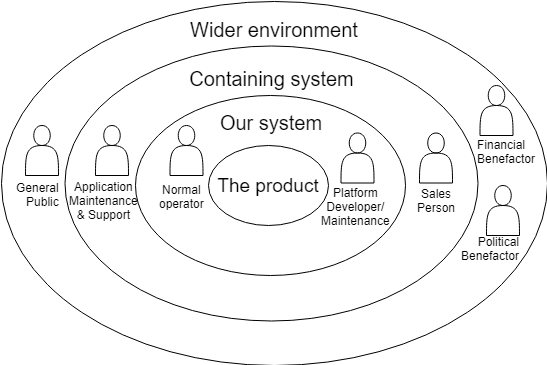
\includegraphics[width=.7\textwidth]{resources/img/onion.png}
\caption{Visual depiction of application of onion stakeholder model}
\label{fig:onion}
\end{figure}
%TODO refs naar chapters waar de informatie gebruikt wordt
%\section{Quality of Service \& Quality of Information}
%TODO write
%\subsection{Quality of Service in WSN} 
%Existing platforms?
%\subsection{WSN energy conservation methods} 
\section{Quality of Information of WSN data}
\label{sec:back:qoi}
In WSNs and IoT applications there is the concept of Quality of Information (QoI). QoI describes parameters depicting quality attributes of information presented by and derived from as system. It is especially applicable to WSNs as they present raw low-level which is then highly processed by subsequent applications. Therefore, the concept of QoI will be employed to validate and evaluate the processing architecture presented in chapter \ref{ch:architecture}. V. Sachidananda et al \cite{qoi_definition} identify the following attributes describing Quality of Information.
\begin{description}
\nospace
\item[Accuracy] The degree of correctness which provides the level of detail in the deployed network. It is the value which is the close imitation of the real world value.
\item[Precision] The degree of reproducibility of measured values which may or may not be close (accurate) to real world value.
\item[Completeness] The characteristic of information which provides all required facts for user during the construction of information.
\item[Timeliness] An indicator for the time needed when the first data sample is generated in the network till the information reaches the target application for decision making.
\item[Throughput] The maximum information rate at which information is provided to the user after raw data collection.
\item[Reliability] The characteristic of information, in which information is free from change or no variation of information from the source to the end application.
\item[Usability] The ease of use of information that is available after raw data collection has undergone processing and can be applied to the application based on user's evolvable requirements.
\item[Certainty] The characteristic of information from the source to the sink with desired level of confidence helping the user for decision making.
\item[Tunability] The characteristic of information, where the information can be modified and undergo processing based on user's evolvable requirements.
\item[Affordability] The characteristic of information to know the cost for measuring, collecting and transporting the data/information. It is the expensiveness of information
\item[Reusability] The characteristic of information, where the information is reusable during its lifetime or as long as it is relevant.
\end{description}
\section{Constraint programming and solving}
\label{sec:back:constraint}
Chapter \ref{ch:rdm} will employ the concept of constraint programming and constraint solvers. The concept of constraint programming encompasses modelling a problem by means of a collection of correlated variables and associated value domains. The relations between variables are captured in a list of constraints. The problem is then solved by finding assignments for each variable with respect to their domains which conforms with the specified constraints

An example of a problem modelled as constraint problem is an automatic sudoku solver. The model would be a list or matrix of integer variables, with each entry having a domain $\{V_i|1\leq V_i\leq 9\}$. The associated constraint would then be $V_1 \neq V_2$ for every combination of entries $(V_1,V_2)$ in the same row, column or 3-by-3 grid.

Several methods exist in order to solve a combinatorial constraint problem. The first and simplest is to perform a brute force search over the solution space. This would produce the Cartesian product of the domains of all variables ($\prod_{i\in I} D_i$) and test them against the constraints. Candidate solutions are rejected until a valid composition of variable assignments is found. This is however a very inefficient procedure as it has to search though the entire search space without optimization. For large combinatorial problems this search space grows exponentially. For instance, for the sudoku example with 20 values filled in, the solution space has a size of $9^{61}(\approx 1,6\cdot 10^{58})$.

A more efficient search algorithm is presented by backtrack-search. Whereas the brute force approach assigns every variable a value and then checks its validity, the backtrack-search algorithm operates on a subset of the variables assigned. By incrementally assigning values to variables it performs a systematic Depth First Search through the search space. If a partial assignment is determined to violate the set of constraints, the algorithm will reject the entire remainder of the search tree. In this manner the algorithm optimizes failing variable assignments by attempting to identify them earlier. For the example of the sudoku solver this entails that an assignment of a 3 to a position adjacent to another square with a 3 will immediately halt the exploration of that branch of the search tree, without the need to consider subsequent variable assignments. It will instead backtrack through the tree by rolling back assignments and attempt a different assignment.

The backtrack-search algorithm can be improved upon further by implementing constraint propagation. This technique attempts to prune invalid variable values from the domain before they are assigned by the backtrack-search algorithm. For example if a square in the sudoku is assigned a three, then the effect of this assignment will be propagated by pruning the number 3 from the domains of every entry in the same row, column or 3-by-3 grid. This eliminates inconsistent options that would violate the constraints before they would be assigned. Additionally, the concept of local inconsistency can be extended to variable domains without requiring any assignment. For example, given two variables $V_1$ and $V_2$ with domains $D_1=\{1,2,3\}$ and $D_2=\{2,3,4\}$ and the constraint $V_1 \geq V_2$, then the values 1 and 4 can be pruned from $D_1$ and $D_2$ respectively. For they are inconsistent with any of the values in the opposing domain and can therefore never validate the constraint \cite{constraint_general, constraint_algorithm}.
%\section{Design Methods}
\section{Commonality/variability analysis}
\label{sec:back:cv_analysis}
In order to design for the problem domain it will require conceptualization. The problem domain(s) will be conceptualized by means of a commonality/variability analysis (C/V analysis). Whereas this analysis is usually performed during the process of system decomposition in product line engineering, it can also be employed to identify common and varying concepts in a problem domain. This analysis identifies the commonalities (invariants) that may be assumed fixed and may be depended upon and the variations in the problem domain which will need to be accounted for by the solution.

J. Coplien et al \cite{cv_analysis} describes the process of a commonality/variability analysis in five steps.
\begin{enumerate}
\nospace
\item Establish the scope: the collection of objects under consideration.
\item Identify the commonalities and variabilities.
\item Bound the variabilities by placing specific on each variability.
\item Exploit the commonalities.
\item Accommodate the variabilities.
\end{enumerate}

The performed conceptualization of the problem domain will mostly focus on step 2 in which a list of common definitions, shared commonalities and variabilities will be provided. Also, steps 4 and 5 will be combined by formulating a list of requirements for intended solution, based on the identified commonalities and accounting for the found variabilities

%\subsection{Design Science Methodology}
%\label{sec:back:dsm}
%TTODO write
\section{Example case}
\label{sec:example_case}
Throughout this thesis the solutions will be demonstrated by applying them to a hypothetical case. Though this case may sometimes seem oversimplified and nonsensical, it does provide an elementary example to illustrate all facets of the solutions without overcomplicating the case. This case is expressly not intended to demonstrate the capabilities or utility of the proposed solution. For that purpose, an application to a more complex real-world case will be performed in section \ref{ch:validation}

The proposed case encompasses an enormous network of low power devices sensing for meteorologically anomalous events. These sensors perform measurements on a regular interval and transmit the measurements to a cell tower to be forward to a back-end application for further processing. For the best results devices should measure and transmit as much as possible. However, since these sensors are not very powerful and employ a limited power supply they will require pacing.

The behaviour of the sensors is typified by two parameters: the sensing interval and transmission interval. Intuitively, it can be stated that shortening either or both of the intervals will result in more fine grained reporting, but will increase the power consumption of the device. Additionally, over time several types of sensors have been deployed with different power sources. Therefore, the amount of electrical power a sensor can use during a given time needs to be restrained in accordance with the specification of its power source and expected life time. Finally, sensors in areas of high interest will require a shorter polling interval, as to gain the most precise information. However, given that the sensor performs the adequate amount of measurements and does not consume more power than it is specified to use, it should measure and report as much as possible.

As for monitoring, the most interested metric is the measurement rate averaged over all sensors. Additionally, it is required to pro-actively monitor the trend of the total bandwidth used by the sensor application. The reason for this is that a constant rise in data rates may ultimately violate the data consumption limits agreed upon with network service providers.

To summarize, a sensor must:
\begin{itemize}
\nospace
\item not consume more power then it is allowed according to its battery specification,
\item measure at least as much as is specified according to the area of interest it is in, and
\item generally try to measure and report as much as is allowed by the previous two requirements.
\end{itemize}
Additionally, the following data points must be provided:
\begin{itemize}
\nospace
\item The average polling rate, and
\item whether the data rate of the sensor application rises consistently for a certain amount of time.
\end{itemize}

In order for the server to determine the intended behaviour of the device and calculate the level of service provided by the application, the following data to be provided to the monitoring application:
\begin{itemize}
\nospace
\item the required measurement rate,
\item the maximum power provided by the power source,
\item the measurement rate of the sensor device, and
\item the bandwidth used by the sensor 
\end{itemize}
Each of these data points stipulates the behaviour of a single sensor at a certain instant. Notice that some data points are normally inferred from raw basic data by auxiliary processes (e.g. required measurement rate). For simplification of the demonstrations these processes are omitted and these parameters are presumed known as a message enters the monitoring application.



%TODO architecture vs. topolgy (at least define definition)
%TODO message vs snapshot
\newcommand{\archid}{1}
\chapter{Design of IoT monitoring platform architecture}
%What needs to be monitored: sensor-networks/IoT 
%How data and information streams flow and combine 
%will focus on data sources and streams as to ascertain which architecture, configuration and components are needed/suitable.
In this chapter we will explain the process taken in order to device our general platform and its architecture. We will accomplish this by first exploring the general problem domain. We will then demonstrate why existing IoT monitoring platforms do not provide the services we require. We will then deliberate the design of our proposed platform and its implementation by identifying the available supporting technologies, clarifying the adaptations made to those technologies and explaining further implementation details. We will then conclude by discussing the success, applicability, disadvantages and deficits of our proposed solution.
\section{Goal}
Large sensor applications send immense amounts of low-level raw monitoring data that requires capturing and enrichment. Individual messages of raw data might contain very little information. However, these messages contain the potential from which meaningful conclusions can be derived, either on single sensor scale or about the sensor application as a whole. This raw data is enriched by combining and analysing datasets of similar, relevant data, in order to achieve a higher level of information. The goal of the efforts described in this chapter is to conceive a software platform that enables software developers to construct their own sensor application monitoring system. We intend to do this by devising a generic application backbone and base building blocks for  developers to extend and compose.  
\section{Conceptualization of the problem domain}
In this section we will investigate the problem domain in order to eventually determine the requirements for the model. We will achieve this by performing a commonality/variability analysis (C/V analysis) \cite{var_invar} of the problem domain. This analysis consists of three concepts:
\begin{itemize}
\item The definitions that will be used in the analysis and the remainder of this chapter, 
\item the common features of all elements in the problem domain which we may assume as established concepts, and 
\item the variations that occur between aspects of the problem domain for which we will need to account for in our proposed solution. Each point of variance needs to be accounted for in the requirements to be established.
\end{itemize}
\subsubsection*{Definitions}
We will start by defining some key terms that we will use in the analysis and the remainder of this chapter.
\begin{description}
\nospace
\item[Platform:] the monitoring platform to be designed.
\item[Application:] the application that is being investigated by the platform.
\item[Snapshot:] a message containing a collection of data-points indicating the state of a system on a certain instant.
\item[Source:] an entity emitting a snapshot. This can be a physical external device or an internal process.
\item[Consequence:] an action taken by the platform based on the analysis of one or more snapshots.
\end{description}
\subsubsection*{Commonalities}
With the definitions established we will continue to identify some common features shared by each application in the problem domain. These commonalities may be presumed during the design of our platform and grants focus to our efforts.
\begin{enumerate}[label=C\archid .\arabic*]
\nospace
\item \label{c:scale_sensor} The group of target applications involves a huge amount of sensors ([scale] which entails a high throughput of snapshots sent and requiring analysis by the platform.
\item \label{c:snapshot} As mentioned in the definitions data is captured in snapshots. These represent the state of (a part) of the application as measured or determined at a certain point in time. These snapshots can be used for both input of the platform as for representing intermediary states.
\item \label{c:snapshot_transformation} The parameters and values of a snapshot, and therefore consecutive derived values, may be considered fixed. Parameters can only change with the introduction of a new snapshot, not during evaluation of the current one.
\end{enumerate}
\subsubsection*{Variabilities}
Finally we will explore the variety within our problem domain. As the purpose of our solution is to process information we will mostly focus on the variables in the domain of information. Our solution should provide proficient adaptability in order to account for this variability. We ensure this by captivating these variations in requirements.
%TODO iets over QoI and information real-estate/capacity
\begin{enumerate}[label=V\archid .\arabic*]
\nospace
\item \label{v:qoi} the first variety we encountered is the variation in Quality of Information (QoI). As described in section \ref{sec:back:qoi} there are many parameters characterizing the QoI of data and QoI can vary on any combination of them.
\item \label{v:conclusion_basis} Secondly, there is the information base on which conclusions are made. The identified conclusion bases are:
\begin{enumerate}
\nospace
\item Single snapshot. (e.g. a sensor requiring maintenance)
\item Multiple sequentially relevant snapshots from a single source. Used to analyse tendency of parameters. (e.g. a sharp continuous increase in bandwidth used which may imply future capacity issues.)
\item Many multi-source snapshots without individual significance. E.g: while the individual throughput of sensors may be of little interest, knowledge of the average throughput of the system may be warranted.
\end{enumerate}
\item \label{v:consequence} The possible consequences by the platform have a large range of implementations and cannot be fully anticipated. Though the exact implementation of consequences can never be exactly anticipated, we can identify some groups of consequences.
\begin{enumerate}
\nospace
\item Build a model for reporting purposes. In order to generate reports some high-level information data-points need to be calculated based on (possibly multiple sequential) large datasets. these data-points are then exposed either by an in-memory component with an API or by persisting it to intermediary permanent storage.
\item Analysis which invokes an immediate feedback response to the application or a command \& control service administrating the application.
\item Alerting or reporting according to a specified rule. When this user defined rule is met or violated an alert is sent to an employee or auxiliary system.
\end{enumerate}
\end{enumerate}
%TODO confirm estiblishment in paper!
The final variety is the scale of the application. We have already established that the platform will operate on applications of large scale, i.e. thousands of sensors. However given a thousand as lower bound, the upper bound is still uncertain. therefore the size of the application is still uncertain and differing degrees of size require different computational needs.
\begin{enumerate}[label=V\archid .\arabic* , resume]
\nospace
\item \label{v:scale} The scale of large wireless sensor applications varies wildly. This yields for both the number of devices in the application and the rate at which the devices send data.
\end{enumerate}
\section{Requirements for the proposed software platform}
In this section we will describe the requirements for the proposed platform, in accordance with the variability identified in the previous section. 
\begin{enumerate}[label=R\archid .\arabic*]
\nospace
\item \label{r:snaptshot_transformation} The platform should enable the capture and transformation of snapshots.
\item \label{r:basis_single} The platform should enable processing of single snapshot.
\item \label{r:basis_historic} The platform should enable processing of a limited window of homogeneous snapshots.
\item \label{r:basis_accumulated} The platform should enable processing and aggregation of an enormous amount of snapshots.
\item \label{r:consequence} The platform should enable implementation of a wide range of consequences. It should at least provide for these anticipated types of consequence:
\begin{itemize}
\nospace
\item model building
\item application feedback
\item rule-based alerts
\end{itemize}
\item \label{r:scale} the platform should be scalable in order to support any large amount input devices
\end{enumerate}

\subsubsection*{Justification}
We will conclude this section by justifying the identified requirements according to the earlier performed C/V analysis. A formal traceability between the requirements, commonalities and variability is listed in table \ref{table:3_justification}

\begin{table}[H]
\centering
\begin{tabular}{|l|l|} \hline
Requirement & Commonality/variability  \\ \hline
\ref{r:snaptshot_transformation} & \ref{c:snapshot}, \ref{c:snapshot_transformation}, \ref{v:qoi} \\ \hline
\ref{r:basis_single} & \ref{v:conclusion_basis}a \\ \hline
\ref{r:basis_historic} & \ref{v:conclusion_basis}b \\ \hline
\ref{r:basis_accumulated} & \ref{v:conclusion_basis}c \\ \hline
\ref{r:consequence} & \ref{v:consequence} \\ \hline
\ref{r:scale} & \ref{c:scale_sensor}, \ref{v:scale} \\ \hline
\end{tabular}
\caption{traceability table for justification of requirements}
\label{table:3_justification}
\end{table}

The first requirements regards the definition and concepts of snapshots and is based on the commonalities and the variation in QoI.  As illustrated by the traceability table the following three requirements closely correlate with the three varieties identified in \ref{v:conclusion_basis}. Requirement \ref{r:consequence} attempts to captivate the variability described in \ref{v:consequence}. This variation is captured in a single requirement as opposed to differenting them (as for \ref{v:conclusion_basis}), because the possible consequences are not limited to the identified consequence groups. Ultimately, the final requirement is regarding the scale of the target applications. This regards both the amount of devices in the target application as the frequency the send their snapshots. 

\section{Exploration of the solution domain}
In this section we will explore the solutions and supporting technologies that are offered to us. We will first consider the base architecture and backbone of the platform, as it is the most fundamental decision to be made. We will then continue to explore the options for message brokers, as a choice for a distributed architecture almost certainly requires one. We will conclude this chapter by examining some distributed cloud computing technologies that should allow us to perform expensive computations by distributing them over a cluster, as to provide the required scalability.
\subsection{Architecture basis and execution platform}
\subsubsection*{Monolithic architecture}
The first option to implement the platform is a monolithic software system. The benefit of such a system is that it keeps the solution as simple as can be. This is illustrated by a famous proverb of Dijkstra: "Simplicity is a prerequisite for reliability"\cite{zoeken}. This simplicity entails a better understanding of the product by any future contributor or user, without the need to consult complex, detailed documentation. However monolithic software products have been known to be difficult to maintain, because code evolution becomes more difficult as more and more changes and additions are made to the code base\cite{TODO:find}. Additionally, monolithic software systems are notoriously difficult to scale up and load balance\cite{TODO:find}, which violates requirement \ref{r:scale}. Therefore we will instead adapt a micro-component approach. Micro-component are  more flexible than monoliths, allow for better functional composition, are easier to maintain and much more scalable\cite{TODO:find}.

\subsubsection*{Apache Storm}
Apache Storm is a big data computing library especially designed for separation of concerns. It performs distributed computing by partitioning the stages of computation. By breaking up the computation, different stages can be distributed among machines and duplicated if need be. The Storm platform consists of three chief concepts.
\begin{description}
\nospace
\item[Spouts:] nodes that introduce data in the topology,
\item[Bolts:] nodes that perform some computation or transformation on data, and
\item[Streams:] connect nodes to one another and allows data to be transferred.
\end{description}
The computation is regarded as a directed graph with bolts as vertices, spouts as initial vertices and streams as edges.

Because data is emitted by spouts individually, Storm can achieve real-time processing of large amounts of data. By breaking up the computations into multiple consecutive bolts, Storm allows computations to be spread over a cluster. Additionally Storm allows individual bolts to be replicated and distributed. This lateral distribution prevents the occurrence of bottlenecks in the network due to bolts executing expensive pivotal processes

Storm is especially suited for our purpose since it was designed for microcomponents connected by streams. In contrast, many micro-component platforms focus on components exposing services which are explicitly invoked by other services\cite{refs: spring, etc}. By employing Apache Storm we obtain both the distributed computation environment as the means of data distribution, simplifying our technology stack.

Conversely however, the built-in stream distribution mechanism is completely internalized, making integration with auxiliary processes difficult. Tasks such as data injection, platform monitoring and data extraction for processing or reporting by third-party programs and stakeholders will require an exposing mechanism. Additionally, Storm requires bolt connections to be explicitly defined at start-up. This causes two disadvantages: Firstly, we cannot update or reconfigure a single process without restarting the entire system. Considerations should therefore be made on when to update the system and when to delay rolling out an updated version. Secondly, the bolts are connected in tuples. This is in contrast to conventional publish/subscribe communication platforms (such as Kafka and RabbidMQ) which decouple the producer and consumers and instead write and read to addressable communication channels called topics. Storm allows reading and listening on streams of a certain topic, but the connection still needs to be explicitly specified. This is cumbersome, but should be able to be overcome. Though cumbersome, this also grants an advantage. With strong component bindings it should prove more difficult to deploy an invalid architecture due to small mistakes as mistypes or not updating all topic bindings on a refactor. 
%TODO iets over real time?

\subsubsection*{Micro-component architecture without execution platform}
A final option is to employ a micro-component architecture without an execution platform. Instead we would deploy components ourselves and have them communicate using message brokers. This would increase the efforts needed to develop and deploy the platform, but does provide greater control over its execution. Additionally this would alleviate the deficiencies identified for Apache Storm, such as difficult third party integration, cumbersome topology building and lack of run-time reconfiguration. 

\subsection{Message brokers}
%\subsubsection{Native HTTP}
%TODO rewrite  to native data transfer
%The Hypertext Transport Protocol (HTTP)\cite{def:http} is a [onmiskenbaar] communication standard this is widely employed in internet communications. It is well-documented and familiar to almost every industry professional, which should [ease] implementation and maintenance. Aside of maintainability HTTP is very versitile, which should ensure that it meets the needs for our system. However, this versitiliy stems from the barebone definition of the protocol. [TODO afmaken]. Additionally, HTTP routing is performed based on the IP address and port of the target process. This requires any sending component to know all its listener components, requiring either direct IP-based subscription or a discovery/lookup service. 
%TODO fast: as fast as consumer/producer
By employing a micro-component architecture we need to identify a communication technology for components to communicate to each other. This approach employs a service to which producers write messages to a certain topic. Consumers can subscribe to a topic and consequently read from it. This obscures host discovery, since a producer need not know its consumers or vice versa. This routing is instead performed by the message service. The following will explore the two widely used message broker services in the industry: RabbidMQ.

\subsubsection*{RabbidMQ}
RabbidMQ\cite{web:rabbidmg} is a distributed open-source message broker implementation based on the Advance Message Queue Protocol. It performs topic routing by sending a message to an exchange server. This exchange reroutes the message to a server that contains the queue for that topic. A consumer subscribed to that topic can then retrieve it by popping it from the queue. Finally, an ACK is sent to the producer indicating that the message was consumed. The decoupling of exchange routers and message queues allows for custom routing protocols, making it a versatile solution. RabbitMQ operates on the \emph{competing consumers} principle, which entails that only the first consumer to pop the message from the queue will be able to consume it. This results in an \emph{exactly once} guarantee for message consumption. This makes it ideal for load-balanced micro-component applications, because it guarantees that a deployment of identical services will only process the message once. It does however make multi-casting a message to multiple types of consumers difficult.
%TODO refs

\subsubsection*{Apache Kafka}
Instead, Apache Kafka \cite{web:kafka} distributes the queues itself. Each host in the cluster hosts any number of partitions of a topic. Producers then write to a particular partition of the topic, while consumers will receive the messages from all partitions of a topic. Because a topic is not required to reside on a single host, it allows load balancing of individual topics. This does however cause some QoS guarantees to be dropped. For example message order retention can no longer be guaranteed for the entire topic, but only for individual partitions. Kafka, in contrast to RabbidMQ's competing consumers, operates on the \emph{cooperating consumers} principle. It performs this by, instead of popping the head of the queue, a consumer retains a counter pointing to its individual head of the queue. This allows multiple consumers to read the same message from a queue, even at different rates. The topic partition retains a message for some time or maximum number of messages in the topic, allowing consumers to read a message more then once. Ensuring that load-balanced processes only process a message once is also imposed on the consumer by introducing the notion of consumer groups. These groups share a common pointer, which ensures that the group collectively only consumes a message once. This process does not require an exchange service, so Kafka does not employ one. This removes some customization of the platform, but does reduce some latency. Lastly, Kafka does not feature application level acknowledgement, meaning that the producer cannot perceive whether its messages are consumed.
%TODO refs

\begin{table}
\centering
\begin{tabular}{|l||c|c|}\hline
  					& RabbidMQ 			& Kafka 		\\ \hline 
Speed				& + 				& ++ 			\\ \hline
Scalable			& +					& ++	 		\\ \hline
Multi-cast			&\xmark				& \cmark		\\ \hline
Multiple reads		&\xmark				& \cmark		\\ \hline
Acknowledged		&\cmark				& \xmark		\\ \hline
Delivery guarantee	&\cmark				& \xmark		\\ \hline
Consumer groups		&\cmark				&\cmark			\\ \hline
Retain ordering		&Topic level		& Partition level\\ \hline
Consumer model	 	&Competing			& Cooperating	\\ \hline
\end{tabular}
\caption{Summary comparison of RabbidMQ and Kafka}
\label{table:rabbidmq-kafka}
\end{table}

 

\subsubsection*{Comparison}
A comparative summery of both technologies is given in table \ref{table:rabbidmq-kafka}. Following this comparason we have chosen to employ Kafka for our platform. The first observation is that Kafka performs better in non-functional metrics. Sources report Kafka to be 2-4 times faster than RabbidMQ\cite{speed_kafka} and the partitioned topics allow Kafka to be distribute and scale overloaded channels. Secondly, the cooperating consumer model Kafka is based on allows us to natively multicast messages to multiple consumers, while still being scalable by defining consumer groups. By choosing for Kafka we do however default some features such as producer acknowledgement and topic level order guarantees. As for producer acknowledgement we do not require it, as producers simply send messages into the clear and consumers are required to make efforts that it processes all data. Using the feature to read messages more than once, we should be able to build a dependable platform. Finally, Kafka cannot guarantee the read order of partitioned topics. We therefore will need to enforce it ourselves in the platform and implementations of it. This can be either done by sorting messages in buffers on some ordered parameter (e.g. timestamp or sequence number) or by not partitioning topics containing order-critical streams.


\subsection{Distributed computing}
As specified by requirement \ref{r:basis_accumulated} we require a means of processing large amounts of data. We accomplish this by aggregating large numbers of snapshots into a distinct smaller amount of snapshots with higher-degree of information. In order to accomplish this we require a scalable means of computation (requirement \ref{r:scale}) 
\subsubsection{MapReduce}
MapReduce\cite{web:mapreduce} is a distributed computing framework. It operates by calling a \emph{mapper} function on each element in the dataset, outputting a set of key-value tuples for each entry. All tuples are then reordered, grouped by key as a key-value set tuple. The key-value sets are then distributed across machines and a \emph{reduce} function is called to reduce the many individual values into some accumulated data-points. The benefit of this framework is that the user need only implement the \emph{mapper} and \emph{reduce} functions. All other procedures, including calling the mapper and reducer, are handled by the framework. An example of the algorithm on the WordCount\cite{search} problem is illustrated in Figure \ref{img:mapreduce}.

The concept of a mapped processor is of a large benefit to our platform. In the early exploration phase it quickly became apparent that there were many use cases where one might want to extract accumulated snapshots per individual sensor or grouped by cell tower. This approach also allows to compensate for groups of devices sending more data then others. These devices would be overrepresented in the population if we did not account for them sending more messages than others. By first grouping the messages per device ID we can assure that every device has the same weight when we, fore example, calculate summations or averages.

\begin{figure}
\centering
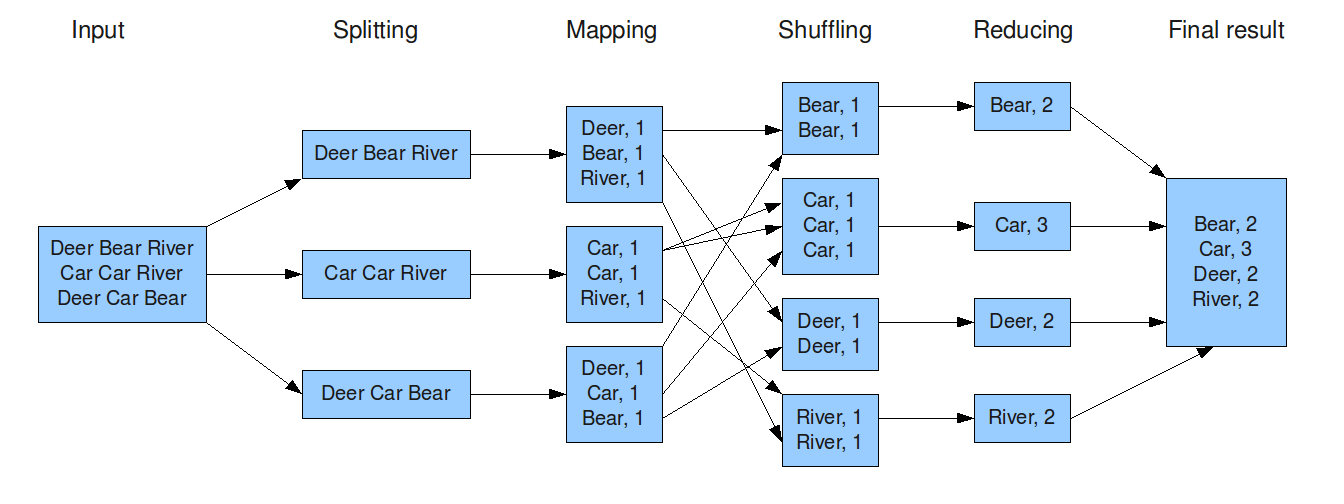
\includegraphics[width=\textwidth]{resources/img/mapreduce.png}
\caption{The overall MapReduce word count process\cite{mapreduce_img}}
%https://www.todaysoftmag.com/article/1358/hadoop-mapreduce-deep-diving-and-tuning
\label{img:mapreduce}
\end{figure}

Though the ease of implmenetation is very high and the technology is very appliccable to our platform, the algorithm has prooved to be comparatively slow. The reason for this is that before and after both the map and reduce phase the data has to be written to a distributed file system. Therefore though highly scalable, the approach suffers by slow disk writes\cite{mapreduce_vs_spark}. Finally, MapReduce works on large finite datasets. Therefore we need to manually preprocess stream data into batches in order for MapReduce to be applicable\cite{stream mapreduce}.

\subsubsection{Apache Spark (Streaming)}
Apache spark is an implementation of the Resiliant Distributed Dataset (RDD) paradigm. It entails a master node which partitions large datasets and distributes it among its slave nodes, along with instructions to be performed on individual data entries. Operations resemble the functions and methods of the Java Stream package \cite{java_stream_handleiding}. 

Three sort of operations exist: narrow transformations, wide transformations and actions. \emph{Narrow transformations} are parallel operations that effect individual entries in the dataset and result in a new RDD, with the original RDD and target RDD partitioned equally. Examples of such functions are \emph{map} and \emph{filter}. Because these transformations are applied in parallel and partitioning stays the same, many of these transformations can be performed sequentially without data redistribution or recalling the data to the master. \emph{Wide transformations} similarly are applied on individual dataset entries, but the target RDD may not be partitioned equal to the original RDD. An example of such a transformation is \emph{groupByKey}. Since elements with  he same key must reside in the same partition, the RDD might require reshuffling in order for computation to continue. Finally, Actions, such as \emph{collect} and \emph{count} require all data to be recalled to the master and most of the calculation is performed locally, resulting in a concrete return value of the process. RDD's provide an efficient distributed processing of large datasets, that is easy to write and read. However careful consideration must be given to the operations and execution chain in order to eliminate superfluous dataset redistribution.
%TODO refs

\begin{small}
\vspace{8px}\hrule
\begin{lstlisting}[
language=Java,
caption=MapReduce example of Figure \ref{img:mapreduce} in Spark RDD.,
captionpos=b, 
escapeinside={(*}{*)}, 
columns=flexible,
numbers=left,
tabsize=4,
breaklines=true,
label=list:mapreduce_spark-search
]
// assumes initial RDD with lines of words = lines
JavaRDD<String[]> wrdArr = 				lines.map(l->l.split(" "));
JavaRDD<String> words =					wrdArr.flatMap(arr -> Arrays.toList(arr));
JavaRDD<String, Integer> pairs =		words.mapToPair(x->(x,1));
JavaRDD<String, Integer> counts = 		pairs.reduceByKey((a,b) -> a+b);
Map<String, Integer> result =			counts.collectAsMap();(*\vspace{5px}\hrule*)
\end{lstlisting}
\end{small}

It is interesting to note that the MapReduce framework can easily be reproduced in Spark. this is achieved by calling the \emph{map} and \emph{reduceByKey} consequtively. To illustrate we implemented the MapReduce procedure of Figure \ref{img:mapreduce} in Apache Spark using Java in Listing \ref{list:mapreduce_spark-search}. Please note that the individual assignments of the RDD are not required. RDD-calls can be chained after one another, but intermediate assignments have been used to better illustrate the steps taken. Also note that the first there steps are be performed fully parallized since they are all narrow transformations. Only line 5 (wide transformation) and 6 (action) require RDD redistribution.\cite{web:user_manual}
% ref e.g.: https://jaceklaskowski.gitbooks.io/mastering-apache-spark/spark-rdd-transformations.html

Additionally, the framework does not require disk writes (as MapReduce does). Instead, it runs distributed calculations in-memory, thereby vastly improving the overall calculation speed. This does however raises a reliability issue, because if a slave node fails it cannot recover it's state. This is resolved by the master by replicating the part of the dataset from the intermediate result it retained and distributing it among the remaining slave nodes. Because the sequence of transformations is deterministically applied to each individual entry in the dataset any new slave node can continue calculations from that point.\cite{web:fault_tolerance}

Finally however, Apache Spark suffers the same deficit as MapReduce and is performed on finite datasets. Therefore streams need to be divided in batches in order to perform calculations. In fact a Apache Spark library exists (Apache Spark Streaming\cite{web:spark_streaming}) which performs in this manner. It batches input from streams on regular, pre-specified time intervals and supplies it to a Spark RDD environment. The time windows can be as small as a millisecond, therefore it is not formally real time, but can achieve near-real-time stream processing.

%TODO integration of communication techniques


\subsection{Solution decision}
\label{sec:solution_decision}
%TODO why niet jar-based with pub/sub
For distributed component platform we have chosen to build upon Apache Storm. The reason for this was primarily that Storm was conceived with this type of real-time streaming micro-component application in mind. The spouts and bolts provide us with the perfect building blocks to design an iterative information refinement application with separation of concerns in mind, while the built-in streaming mechanism provides the needs for a real-time distributed application. We will however need to account for the lack of expose points for third party integration and the tedious process of specifying each and every bolt connection.
%TODO meer meer meer. storm is awesome

Though Storm contains the means for large scale snapshot aggegation, we will not employ it. Instead we will base our data aggegation on Apache Spark Streaming. The reason for this is that studies have shown Apache Spark to be 5 times faster than both MapReduce\cite{spark-vs-mapreduce} and Storm\cite{spark-vs-storm}. Spark does however have a larger latency, due to collecting batches of data instead of processing them real-time. This however should not cause a significant problem since our envisioned use case is for timed analysis jobs on very large amounts of input data, in order to detect or visualise collective tendencies of the system under investigation. For this scope of application the latency issues of Apache Spark do not impose a large deficiency.

To facilitate external communication of the platform we will employ Apache Kafka. The reason for this is its speed and greater scalability. Additionally, but to a a smaller degree, this was chosen because of Kafka's ability to multicast messages. This will allow multiple auxiliary processes to listen in on the proceedings of the platform. With our choice for Kafka comes another benefit, as the Spark Streaming library contains adapters for Kafka allowing direct connection to it. Therefore we can simply emit data to a Kafka topic and connect a Spark Streaming process to it. The greatest deficiancy of Kafka, being the lack of topic-level order guarentee, is not of grave importance. The hindrence can be overcome by including timestamps or sequence numbers in the passed messages. Moreover, the Spark calculations most likely will not require order retention. The reaseon for this is that most computations will contain of a \emph{reduce} step, which requires the reduction operation to be both associative and commutative\cite{ass-comm}. Therefore the message order is of no importance.

\section{Design of the software platform}
%TODO java!!!
We will adapt these technologies by composing them using adapters and abstracting the solutions. By abstracting the technologies we shield the internal implementation details, simplifying implementation by the user. We will provide the implementer some scaffoldings for bolts intended for different types of data flows and data reductions. Additionally, these technologies are very abstract since they were intended for many unspecified usages. Since our platform and group of target applications features some known commonalities, which were considered variations when designing the original technologies, we can implement some functions which were originally intentionally left unspecified. This will reduce the implementation effort required, again simplifying usage of the platform. \cite{facade_pattern} 

%TODO onderscheid wanner het gaat over mijn platform en wanneer apache

\subsection{Micro-component architecture}
In the remainder of this section we will explain what adaptations to the previously discussed technologies are made.

\subsubsection*{Apache Storm}
%TODO define 'processor'
%TODO 'define topology ' and why it is cumbersome
%TODO facade pattern obscures/abstracts storm (kan ook hierboven)
The bulk of the component construction and execution, and streaming services of the platform will be performed by Apache Storm. However, as discussed before, the process of specifying a topology in Storm is a cumbersome process due to the necessity of interconnecting each and every process individually. Therefore, cross-connecting $M$ producer components with $N$ consumers requires $M\cdot N$ explicitly specified connections. This is contrasted by technologies that employ topic based channels in which $M$ producers write to a channel to which $N$ consumers are subscribed, requiring but $M+N$ connections to be specified. To this end we have developed a topology builder which enables topic based streaming. The builder will automatically connect the specified components according to the topics they are subscribed to, when executed. In this manner a component and its connections can be specified with but a few lines of code, as demonstrated in listing \ref{list:topologybuilder}. Note that the complexity of the topology does not impact the amount of code needed, as the code complexity is solely depended on the number of components and not how they are interconnected.

\begin{small}
\vspace{8px}\hrule
\begin{lstlisting}[
language=java, 
caption={Declaration of a processor and communication channels}, 
label={list:topologybuilder}, 
escapeinside={(*}{*)}, 
captionpos=b,
numbers=left,
tabsize=4
]
topologyBuilder.declareBolt(new UserDefinedProcessor("pname"))
	.subscribeAsConsumer("sensor_input_channel")
	.declareAsProducer("debug_channel", "output_channel");(*\vspace{5px}\hrule*)
\end{lstlisting}
\end{small}


Since Storm allows processes to be duplicated for load-balancing purposes, it employs some methods of controlling which duplicated process worker will consume which messages. The two chief methods are supported by our platform. The first method is the \emph{shuffle grouping}. It is the simplest channel specification and does not offer any guarantees on which process worker will consume the message. It is therefore described as receiver-agnostic. However this lack of guarantee will not effect most tasks since most will be stateless data processors. The second supported stream manipulation method is the \emph{field grouping}. It is used for processors that do retain a state or somehow require similar messages to always be processed by the exact same worker. An simple example of this is a processor that counts the number of messages received for each sensor in a WSN. If we cannot guarantee that all messages of a sensor \emph{S} are always processed by the same worker \emph{W}, one worker might count 40 messages and another would count 60 of them. This would require another singular processor that accumulates those counts in order to derive an accurate message count. Therefore it is possible to specify a set of fields which will deterministically and consistently determine which worker will consume a message. In our adaptation this is specified at topic level, again to prevent repeated declarations. Therefore each snapshot emitted to such a channel is required to include all fields specified for that channel.

Finally, though we believe the abstractions and encapsulations of the Storm platform to be useful to simplify implementation efforts, it could still be useful to an implementer to inject their own native Storm bolts or spouts. This might be due to reusing earlier defined bolts or requiring more control of a process than our abstraction offers. To this end we have chosen our topology builder to encapsulate the topology builder provided by the Storm Java library. This entails that our topology builder, upon calling the \emph{build()} function, will return an instance of \emph{org.apache.storm.topology.TopologyBuilder}. This allows last-minute injection of self-specified native storm processes, before ultimately generating the Storm topology with that builder.

\subsubsection*{Incorporation of Apache Spark Streaming}
\label{sec:incorporation_spark}
As identified in by requirement \ref{r:basis_accumulated} there is a need to condense the information of enormous amounts of (individually) low-information snapshots into a distinct number of high-information snapshots. Additionally, the large amount of input snapshots, and the assertion that the platform should be scalable (requirement \ref{r:scale}) entails that we should make a scalable data accumulator available. 

As specified in section \ref{sec:solution_decision} we have chosen Apache Spark Streaming for this task. However this causes an earlier identified problem: a direct incorporation of Apache Spark in Apache Storm is difficult. In order to solve this inoperability of interfaces we have chosen to device a process that adopts the adapter software pattern \cite{search_ref}. This adapter employs Apache Kafka, for which Spark does provide interfaces, to pipe snapshots obtained from Storm channels. Snapshots are then read from a Kafka channel and batches of snapshots are fed to Spark RDD computations. Once the cloud computations have concluded the data is returned to the Storm environment and aggregated snapshots are eventually forwarded to consecutive processes. This is achieved by deploying two Storm components. Firstly, a specialized Storm bolt named \emph{KafkaEmitter} is deployed. this process simply consumes Storm messages and forwards them to a Kafka channel. Secondly, a Storm spout is deployed which acts as a Spark master node. This bolt contains the instructions for the distributed computation of the Spark cloud and results of the cloud computations will be returned to it. A graphical representation of this process is depicted in Figure \ref{fig:distributed_accumulator}.

\begin{figure}
\centering
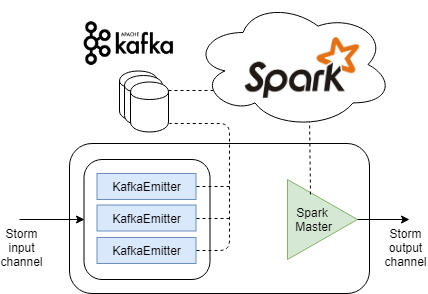
\includegraphics[width=.7\textwidth]{resources/img/distributed_accumulator.png}
\caption{Graphical depiction of the distributed accumulator process}
\label{fig:distributed_accumulator}
\end{figure}

Two interesting remarks should be made, as apparent from Figure \ref{fig:distributed_accumulator}. Firstly, The KafkaEmmitter can be replicated in order to prevent it being a choke-point in the topology. Secondly, the fact that two distinct components (KafkaEmitter and Spark Master) are present is encapsulated by the topology builder. Developers need only declare an implementation of the distributed accumulator processor (acting as Spark master node) with the appropriate Storm and Kafka channels. The builder will then deploy a KafkaEmitter (or several) and the accumulator. This makes deploying the processor easier and obscures the internal implementation by appearing as a single component.

\subsection{Scaffolds for micro-services}
With the supporting technologies established we will now describe and deliberate the component scaffolds that are supplied for application developers by the platform. We will first describe the base functions shared by all components, before discussing them more in depth individually.

\subsubsection*{Common functionality}
Firstly, the components contain all functionality and information required to emit new snapshots to consequent components. A developer need only package the information in a message containing key-value pairs and specify to which stream a snapshot should be emitted. The component then uses the information it received during the building of the topology to route the snapshot to all receivers subscribed to receive it. This not only implies routing the snapshot towards the correct component but also the correct component worker according to the defined field grouping.

Secondly, all components contain a base implementation of the \emph{prepare(args)} \footnote{actual arguments have been omitted due to simplification} method. This method is used to instantiate some properties that cannot be instantiated in the objects constructor. The reason for this is that all components extend some abstract spout or bolt class of Apache Storm. In the Storm platform all spouts and bolts adhere to a pre-specified execution order. The component is:
\begin{enumerate}
\nospace
\item created by one of its constructors,
\item transmitted to one of the slave nodes of the Storm cluster,
\item further instantiated using the \emph{prepare(args)} method, and
\item executed according to its specification.
\end{enumerate}
The reason for this course of action is that step 1 is performed on the Storm master node, before distributing the functional object over the cluster. Therefore, during step 2 the object and its members need to be serializable. Non-serializable members are consequently instantiated during step 3, after the object has been transferred and before functional execution. The \emph{prepare(args)} method thus can be used to instantiate certain user-specified non-serializable properties. However, one should note that overwriting this method also requires invocation of the super method, since the default implementation specifies some non-serializable Storm properties and classes.

\subsubsection*{Spout}
This process is named after to the Apache Storm spout and is the component that introduces snapshots to the network. This component typically contains a handle to some external data source such as a database, API or streaming technology. The reason we need a special processor for this is the special execution cycle it has compared to a Storm bolt. Bolts execute with interrupts. They halt their execution until a new message is available. However, a spout runs on an infinite-loop (until termination) continuously calling a method \emph{nextTuple()}. This method polls, retrieves and emits messages depending on the origin of the source.

\subsubsection*{SingleMessageProcessor}
This component is the most basic scaffold and closely resembles a Storm bolt. It however contains some additional functionality that improve the ease-of-use. It receives a snapshot and performs computations or analyses on it, before emitting new, enriched snapshots. Its typical use is for transformations of individual snapshots. As noted before this component requires implementation of a singular method: \emph{runForMessage(Message\ m)\emph} which will be called for each key-value pair received by the component.

%TODO make indexable by key
\subsubsection*{HistoricBufferedProcessor}
The HistoricBufferedProcessor resembles the SingleMessageProcessor in that it consumes single snapshots, but instead it computes on or analyses a series of sequentially relevant snapshots, called the \emph{window}, sorted by sequence or time. This is performed by retaining an in-memory buffer to which new snapshots are amended and is periodically filtered on relevance. This component can for example be used to analyse and determine recent trends in system parameters. The methods that require implementation for this component are \emph{runForBuffer(List\textless Message\textgreater\ l)}, which is run every time the buffer is updated, and \emph{cleanBuffer(List\textless Message\textgreater\ l)} which implements how and which elements should be pruned from the buffer should they lose their relevance.
%TODO require field grouping?

\subsubsection{DatabaseBufferedProcessor}
TODO

\subsubsection{DistributedAccumulatorProcessor}
This component is used to aggregate large amounts of laterally relevant snapshots. By laterally relevant we mean that the snapshots describe similar data-points, but have no sequential relevance. The input for this process is a large amount of (individually) low-information snapshots in order to emit some high-information snapshots. An example of its usage is combining thousands of snapshots from individual sensors in order to obtain some collective performance parameters. For the task of accumulating and aggregating these enormous amounts of data we employ the accumulator principle described in section \ref{sec:incorporation_spark}. By means of the method \emph{runForRange(JavaRDD\textless Message\textgreater\ rdd)} this component offers implementers a reference to the Spark RDD which contains all the snapshots collected during a user-specified time period. The implementer can then use this RDD reference to sequentially manipulate and aggregate the collection of snapshots. Keeping proper parallelization in mind, this distributed component can perform data enrichment tasks on enormous batches of streaming data.
A final remark to be made is on the granularity of the batch processing. As stated before [(echt?)] some real-time properties are lost by collection and processing streaming data as batches. This has been partly mitigated by employing the windowing mechanism of Apache Spark Streaming. This mechanism collects data in relatively small sub-RDDs. one or more of these smaller consecutive RDD's are then collected as one larger RDD called the 'window'. This window has a fixed size and slides over the sequence of sub-RDDs. This allows these small batches to be part of several consecutive windows. A graphical representation of this process is depicted in Figure \ref{fig:spark_window}. By this method it allows for example the analysis of data windows of the past 5 seconds, every one second. Whereas without this mechanism it would only be possible to process the last 5 seconds every 5 seconds or the last second every 1 second. Additionally, this process is very efficient, since the internal windowing mechanism automatically caches the results of the intermediary sub-RDD's. Therefore the entire chain of computations does not need to be recalculated for each windowed operation, only the transformations past the caching of the sub-results.

\begin{figure}
\centering
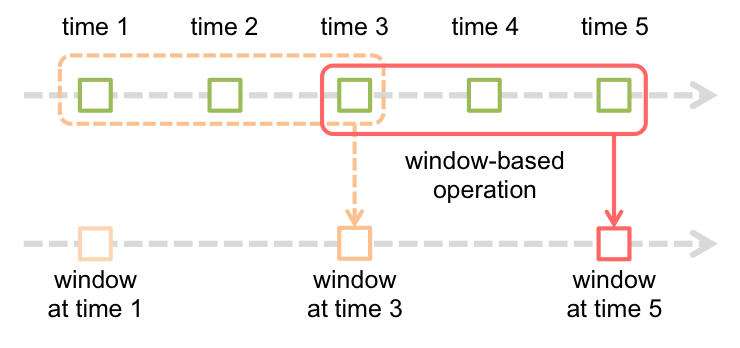
\includegraphics[scale=0.55]{resources/img/spark-window.png}
\caption{Apache Spark windowing mechanism. Source: \cite{spark_user_guide}}
\label{fig:spark_window}
\end{figure}

\subsubsection*{AccumulatorProcessor}
This component closely resembles the function of the above described DistributedAccumulatorProcessor, but is executed locally rather than on a cloud cluster. The purpose of this processor is tasks that would otherwise require the distributed accumulator, but can instead be run in-memory on a single machine. This could be a viable solution for applications that either run the accumulator task often enough or do not collect excessive amounts of snapshots. For these class of applications a locally executed accumulator task should prove sufficient and inclusion of such a components eliminates the base requirement of a Apache Spark cluster to be deployed in order for the platform to be deployed, since the DistributedAccumulatorProcessor is the only component that employs it. It should however be noted that not deploying an accumulator in distributed mode could introduce a bottleneck in a Storm topology since the accumulator cannot be load-balanced. Load-balancing would require a sequential singular component that combines intermediary results aggregated by the load-balanced workers into an eventually final snapshot

To facilitate the easy implementation of the AccumulatorProcessor the processor was modelled after the MapReduce paradigm. An implementer need only specify a series of MapReduce steps (possibly singular) and an eventual single collect step.  The exact methods to implement for this are: 
\begin{description}[font=\normalfont]
\item[\emph{map(Message m) : String}] \hfill \\ Computes the key for a key-value message.
\item[\emph{reduce(String key, List\textless Message\textgreater\ l) : Message}] \hfill \\ Reduces sets of key-value pairs grouped by key determined in the map step.
\item[\emph{collect(Map\textless String,Message\textgreater\ m) : Map\textless String,Message\textgreater}] \hfill \\ Collects the key-message pairs emitted by a reduce step. The return value of this method is a map of messages indexed by the Storm topic on which it should be forwarded.
\end{description}
Please note that the return type for the reduce step is a new message. It is therefore possible to chain multiple map-reduce steps sequentially, as long as the sequence is concluded with a collect step.

\subsubsection*{ResourceDistributionModelProcessor}
%TODO here or in other chapter
[TODO]

\subsection{Demonstration by example topology}
\label{sec:example_application_topology}

\begin{sidewaysfigure}
\centering
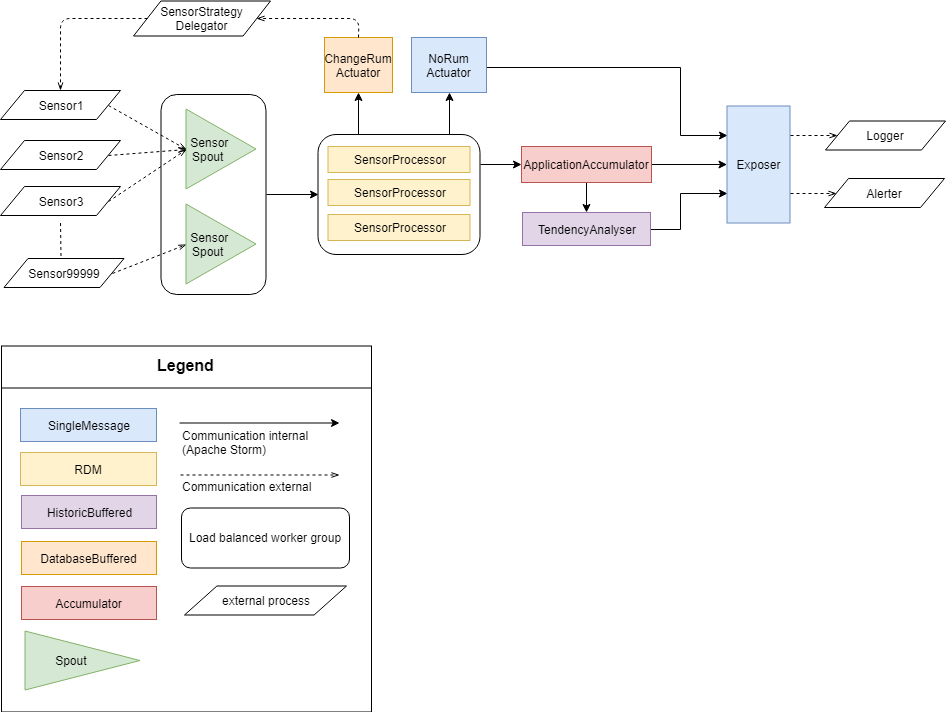
\includegraphics[width=\textwidth]{resources/img/example_topology.png}
\caption{Example topology of a platform implementation according to the example case}
\label{fig:example_topology}
\end{sidewaysfigure}

In this section we will illustrate an example of the composition of the specified components. For this purpose we will consider the case exemplified in section \ref{sec:back:example_case}. A graphical depiction of the topology for the example implementation is found in figure \ref{fig:example_topology}. 

As figure \ref{fig:example_topology} makes apparent, the application encompasses a large number of sensor devices. These devices regularly send their status information to our application via some external communication technology (e.g. Apache Kafka). These snapshots are introduced into our topology by \emph{SensorSpouts}. These spouts have been duplicated in order to accommodate the large amount of sensors which might send a sudden burst of data. The snapshots are then forwarded to the \emph{SensorProcessors} which have been provisioned with a Resource Distribution Model. This model consumes the measured parameters of the input snapshot and uses them to further calculate all the parameters which can be derived from the inputs, according to the specified model. This model also determines the optimal mode of operation for this sensor device. Should no valid model composition be found this is reported to the \emph{NoRumActuator} which forwards a log message to the \emph{Reporter} component. The \emph{Reporter} will delegate the message to the correct reporting/alerting mechanism, outside of the topology. 

Should the current mode of operation be determined not to be optimal, the \emph{SensorProcessor} will report to the \emph{ChangeRumActuator}. The \emph{ChangeRumActuator} will report requests for change to an entity outside of the topology of the application. The actuator has been implemented as a DatabaseHistoricProcessor. The reason for this is that it will recollect the last few messages it received for this sensor and will only actually change the mode of operation of the sensor if it is consistent with the last few messages it received. In this manner we can eliminate superfluous expensive communication with the sensor device due to sporadic behaviour. Alternatively this component could have been implemented as a BufferedHistoricProcessor. However, a sensor is expected to send monitoring data only a few times per day and consequent a changes of operation would occur even less. It would therefore make little sense to keep a buffer of the last messages sent for each and every sensor in-memory. Additionally, this would have required a field grouping in case the component were to be load-balanced in order to enforce that the request for change of a particular sensor always be sent to the correct worker instance.

A final transformation to be performed is to infer application level intelligence from the low level sensor statuses. This is performed by the ApplicationAccumulator which collects data for a certain time period and calculates some high level data points, such as the measurement rate of the application averaged over its sensors, the total throughput and how many devices are performing on which RDM. This information is forwarded to the \emph{Reporter} which will make it available for visualization performed outside of the topology. Additionally the accumulator sends its aggregated snapshot to a \emph{TendencyAnalyser} which keeps a sequence of the total bandwidth during the time windows. Should this total consistently rise over a period of time or over a number of snapshots an alert will be sent by the reporter, as specified by the alerting requirements listed in section \ref{sec:back:example_case}.
	
\section{Discussion of the proposed software platform}
In this section we will evaluate the design of our monitoring platform. 

\subsubsection*{Satisfaction of requirements}
The first order of business is whether the proposed design satisfies the earlier stated requirements. we believe that the message-passing micro-service architecture provides the basis for snapshot transferral and transformation as stated in requirement \ref{r:snaptshot_transformation}. Furthermore, we believe that the requirements \ref{r:basis_single}, \ref{r:basis_historic} and \ref{r:basis_accumulated} are satisfied by the inclusion of the \emph{SingleMessageProcessor}, \emph{BufferedProcessors} and \emph{AccumulatorProcessors}, respectively. Finally, the last two requirements regarding the size of the applications in the problem domain and entailing scalability of the solution have been decisive for many choices of the supporting technologies and are reflected in our employment of cloud processing technology Apache Spark. From the aforementioned arguments we conclude that every requirement is represented and met in the design of the platform.

\subsubsection*{Completeness according to QoI attributes}
The goal of the platform is to process and enrich data. It is therefore rational to evaluate the appropriateness and compleness of the platform by considering the information processing capabilities it offers. In this section we will thusly evaluate the platforms completeness by demonstrating that the platform not only satisfied our identified requirements, but also does not negatively impact the Quality of Information (QoI) of the input data. By this we intend that the QoI is improved or retained, but never lost as data passes through the platforms topology. We will achieve this by arguing the QoI parameters which were enumerated in section \ref{sec:back:qoi}. 

The first consideration of QoI is regarding the processing of data by our platform and affects the precision, completeness and ease of use of information. Firstly, \emph{precision} and \emph{certainty} are obtained by employing the HistoricProcessors. By averaging measurements anomalies are mitigated and the measured value closely approaches the norm of the measurements. Provided that the accuracy of the measurements is sufficient, this improved precision should consistently yield a measurement near the actual value. Secondly, the \emph{ease of use} of information is improved as data moves throughout the topology. To illustrate this we propose a thought experiment using the example topology listed and described in section \ref{sec:example_application_topology} and a batch of raw data emitted in a certain time window. Before the data enters the platform it contains all the information potential to calculate the average throughput offered by the entire sensor application during that time window. Otherwise our platform equally would not be able calculate it. However, actually calculating it would involve extracting the correct data-point(s) from each snapshot, calculating device performance, extracting the throughput, averaging it for each device individually and ultimately calculating the average over the entire application. Instead this process is automated by an implementation of our platform and the resulting information is offered for further processing or visualization. This demonstrates that our platform can facilitate ease of use for information by calculating and producing a ready-for-use value. It should however be noted that the \emph{completeness} of the information is greatly reduced during this process. To illustrate, from the average application throughput the throughput for individual devices can no longer be determined. For this reason, and others which will become apparent, we recommend committing the raw data to storage before processing it.

The second class of QoI attributes regards the processing efforts, expressed in time and costs. As the relevance of information degrades as time progresses timely processing is paramount. We provide \emph{timely} execution by providing a scalable distributed solution. This ensures that, regardless of the intense information \emph{throughput}, the calculations can be performed in near real-time. Notice that we only claim \underline{near} real-time, since Apache Spark collects records during a time window and performs calculations in batches. However the time window of such a batch can be set arbitrarily small and the windowing mechanism of Spark allows for efficient fine grained processing, so it does not impact the timeliness greatly. However, adverse to this gained timeliness we have a decreased \emph{affordability}. In order to incorporate these distributed cloud technologies a cluster of machines and increased development resources will need allocation. When the solution does not require this degree of scalability this poses an undue burden. We have therefore also supplied the locally deployable alternatives to these distributed processors. Implementations of the platform are therefore offered a trade-off between timeliness and cost.
	
Lastly, we have the \emph{tunability} and \emph{reusability} of the information. Firstly, the data can be duplicated among different communication channel which allows differentiating calculations to be performed on the same data. Secondly, in order to facilitate evolution of end-user demands the platform has been designed with separation of concerns in mind. This allows continuous reconfiguration of the platform to be performed with reduced occurrence of concern entanglement. By redeploying the topology the same raw information can be used to facilitate updated user demands. This is also another reason to store the raw data before processing it. By caching the data it can be re-fed into an updated topology in order to initialize an application as if it had been running for days.

Some final remarks should be made on the analysis. Firstly, our platform cannot offer any improvement or retention of information \emph{accuracy}, as it is solely determined by the method and quality of data measurement. Secondly, it should be noted that our platform cannot assure preservation of any of these metrics, since an implementation of the platform can violate any guarantee made. It can only be claimed that the platform does not impede any of the parameters and offers the means for developers to develop applications that do guarantee it.

\subsubsection*{Ease of adaptation}
The first point of focus is the ease of adoptation provided by the platform itself. We believe that by offering some abstract components that require implementation of one or but a few methods, we have effictively obscured the low level implementation details of Apache Storm and Spark. This obscuration entails a clearer programming interface to an implementer, as defined by the \emph{facade} programming pattern. \cite{facade_pattern} 

Secondly, the provided topology builder facilitates easy and fast building of a Storm topology. It does so by providing context aware topology and process instantiation, and topic based communication subscription and emission.  As mentioned before this allows $M$ producers and $N$ consumers connected by a single topic to be connected with complexity $\Theta(M+N)$, instead of the complexity $\Theta(M\cdot N)$ which would be required without the concept of topics. This allows our example topology described in section \ref{sec:example_application_topology} can be specified using only [xxx] lines of code.

\subsubsection*{Technology stack}
The second issue to contemplate is the technology stack required for the platform. As mentioned in section \ref{sec:solution_decision} we chose Apache Storm as enabling technology because it offered most of the features required and would reduce our technology stack. However by employing Apache Spark for distributed data aggregation we have introduced two cloud technologies, as Spark requires Apache Kafka in order to be connected to a Storm Topology. We do however hold the belief that the inclusion of a distributed aggregator is necessary in order to keep the computation scalable. Additionally the speed and efficiency arguments raised in section \ref{sec:solution_decision} justify the deployment of these additional technologies. Finally, when this scalability is not required Apache Spark and Kafka clusters can be executed locally on a single machine, which would still enjoy benefits from process parallelization. Finally Spark and Kafka may be omitted entirely, as a non-distributed data aggregator is also included.

\subsubsection*{Future work}
Finally, our topology-based separation of concern approach allows for visualization of the computations and distribution. The chain of computations can easily be depicted as a directed graph with processors and topics as nodes and processor-topic connections as vertices. Such a topology visualization would for example be very useful for identifying incorrectly or disconnected components. With an even more extensive user interface an editor tool could be device, allowing a topology to be drawn and functional methods to be implemented later. It should be noted that, though promising, the library does not feature such visual user interfaces. However future efforts could be made to facilitate them.

%ease of use
%large technology stack
%qoi metrics
	%datastreams


%ease of use
%	topology build by 2 lines of code per component (4 if formatted)
%		create, register, declare, subscribe
%	total for test topology = xxx
	
%large stack -> also supply old accumulator
%also supply old
%		lower stack
%		gebruikt during development
%		map-reduce
%			rdd not map-reduce
%		Spark can run locally
%???	
%1. Every stream ends in distinct collection/number of streams -> therfore no n*m analysis necessary (only for each stream and for each analysis individually. (htis only descirbes outputs, not the inputs)
%2. there are no one/N to many relations. Implications?
%+RUM

%no mass emitter?
%??


%Discussion aan de hand van qoi metrics

%future work?
%composer GUI?



%architecture
%	model reification
%what components needed
%	featuremodel
%	requirements
%which candidates
%benchmarking
%desicions

\newcommand{\rumid}{1}
\chapter{Resource Distribution Model}
\section{Requirements}
In this section we will [discover] the requirements for the [method of] the RDM. We will achieve this by performing an commonality/variability analysis [ref]. This will [tell] us what the common [features] are which we may [assume] and the variation for which we will need to [design].
\subsection{Commonality/variablity analysis}
\subsubsection{Definitions}
\begin{description}
\item[Resource:] Any measurable/calculable parameter of a system
\item[Component:] Any physical or hypothetical entity that can consume or produce a resource
\item[QoS:] ...
\end{description}
\subsubsection{Commonalities}
\begin{enumerate}[label=C\rumid .\arabic*]
\item Any resource can be consumed or offered by a component
\item A resource can be produced or consumed by multiple components
\item Resources are scarce. I.e. the amount produced must exceed the amount consumed.
\item \label{c:res_transf} Resources are correlated and can converted into one another.
\end{enumerate}

\subsubsection{Variabilities}
\begin{enumerate}[label=V\rumid .\arabic*]
\item \label{v:obvious} Obviously, we cannot predict all resources, constraints and components that might be used.
\item \label{v:micr_macro} Resources of a system can be modelled on a micro-scale or macro-scale.
\begin{itemize}
\item A micro scale (e.g. a single sensor) entails concrete, palpable parameters.
\item A macro-scale (e.g. an entire WSN application) entails accumulated, theoretical parameters
\end{itemize}
\item \label{v:nr_optimizer} A system can have multiple resources as QoS indicators
\item \label{v:granularity} short term resource usage (e.g. seconds) requires a different granularity than long term resource usage (e.g. interval in days).
\item \label{v:measure_vs_derive} Some resources are directly measurable and thus [fixed] for a certain moment of measurement. However, some resources are derived and calculated using other resource values. \cite{feature_model}
\item \label{v:state} Most resource values differ depending on system's measured state
\item \label{v:function} Some resource values differ depending on a specific system function
\end{enumerate}

\subsection{Requirements}
\begin{enumerate}[label=R\rumid .\arabic*]
\item \label{r:main} The model should represent resource distribution in a system
\item \label{r:transform} Resources should be able to be transformed into other resources (many-to-many)
\item \label{r:resource_types} The model should account for the fact that the value of a resource can originate from different sources. These sources are the following (accompanied with an example):
\begin{description}
\item[constant] a predefined value specified on development time (e.g. initial battery capacity),
\item[measured] a value specified as observed on evaluation time (e.g. percentage of battery capacity left),
\item[calculated] derived from measured values (e.g. runtime left),
\item[variable] any value or a calculation depending on specific system function (e.g. power usage).
\end{description}
\item \label{r:optimizer} Each model should have one, and only one, resource that is associated with a heuristic optimizer function.
\item \label{r:calculable}Given a resource distribution model, constant-valued resources and measurements, for each combination of values for variable resources, a value should be able to be evaluated for each calculated resource
\item \label{r:solvable} Given a calculable  resource distribution model (\ref{r:calculable}), a set of resource constraints and an optimizer function; an optimal, valid appointment for each variable resource value should be able to be solved efficiently.
\end{enumerate}

\section{State-of-the-art}
[Some] work regarding modelling resource [distribution has been performed in several studies. An elementary example of such research is the studies of [name][ref]. Through their efforts they [layed] the ground work for representing entities interconnected by shared resource. This UML-based model was one of the first examples of such a representation using formal [principals]. Another example of early research is the study performed by [name][ref]. This study focussed on modelling resource utilization in embedded systems using timed state machines. The transitions in these automata were attributed resource costs to model the consumption of resources for remaining in a state or transitioning to another. [Possible] resource consumption and performance could then be calculated and analysed. 
A continuation of this work was performed by [lalala] et al [ref]. They [combined] the approaches of the previous authors by provisioning the modelled software/hardware components each with their own state machine. These state machines model the resources and services that are offered and required by the components. By [extracting/analysing] these component models as composite state machines, model checking tools (such as UPAAL [ref], [more?]) can be used to analyse and evaluate the performance of the system under investigation.
%TODO voorbeelden hebben maar 1 RUM

\section{Solution}
\subsection{Solution options}
These efforts have produced suitable methods of representing components connected by shared resources. Espesially the notation of [name 3e][ref] which is both intuitive and [descriptive]. We will therefore continue to use this notation throughout this [paper]. 
however these models are all focussed on components that are self-aware of their resource usage and performance. Instead, we are interested in [off-site] analysis of interconnected resources and accumulated performance of the entire system. Our focus is therefore alternatively more resource-centered. It is concerened how production and consumption of a resource is interconnected, with components serving as secondary [elements] merely specifying how these resources are converted to other resources. Therefore a resoucre-centered adaptation of this framework might be more suitable for our problem.
%TODO meer

Secondly, there is the issue of how to [represent] the RUM, the model for variable behaviour of components. Previous [attempts] [refs] have used timed automata to represent behaviour cycles. This allows for automated tools to calculate a runtime schedule in [incredable] levels of granulrity. However the high level of granularity comes at the cost of efficiency. When we shorten the [time] interval the [system] requires additional time and computational resources. This might [impose] a problem on resource constraint devices or applications that require the [program] to run many times for [many] [devices/systems]. Additionally, we need to consider that a component might be able to operate according to differing RUM'S for which a valid, optimal RUM needs to be determined. In the worst [case] these RUM's [influence] each other, which implies that for each composition of models the individual models need to be re-evaluated [%TODO validate]. 

An alternative approach is to model the RUM as a flat set of paramters. This is achieved by averaging the behavour otherwise modeld by timed automata. This comes at great cost of granularity, since the RUM's now only describe static, long-term behaviour. However it significantly improves the complexity of the search space, since the only exponential factors are the number of variable components and the number of RUM's for those components. For this approach timed automata is no longer a sensible technology since the element of time intervals has been eleminated. Instead the problem is pure decision [beter uitleggen, ref] which's search space can be explored with a simple brute force search. However more effectively, combinatorial problems can often be solved with constraint solvers. The problem is easily [transposed] to a constraint problem with the resources as model, resource constraints as constraints and the RUM's as variables for the variable components. With the many solution strategies described in \ref{subsec:constraint} available for different types of problems, a suitable solver must be [possible].

\subsection{Solution choices}
With careful consideration the following choices for the solution implementation have been. For modelling we chose to [adapt] the framework of [ref] by emphesizing on resources. This allows constraints to be [added] to resources, modelling the limits and requirements of the system. The components will still exist in the model, but will merely serve the function of connecting two ressources to one another. Another adaptation is the existence of multiple RUM's for a component, which allows calculation of the optimal system functionality.

As for who to model the RUM, we chose to reduce the complexity of the system by modelling variable resource usage with static parameters. The strongest advocate for this choice is the fact of the focus for this research: large IoT applications. In an IoT monitoring platform the RUM [determination] process will need to be performed repeatedly for many sensor devices. Additionally, most IoT [refs!!!] devices only send and recieve data a few times per day. Therefore high granularity is not of grave importance because the feedback-control cycle is not that short. However, eventhough we do not use timed automata at runtime, they are still a valueble technology to be used when developing and testing the static parameters a RUM at develop-time. The choice for static RUM's implies constraint programming as a suitable model solver paradigm. 

\section{Design}
\subsection{Model}
A graphic representation of the adapted metamodel can be found in figure \ref{fig:component}. To illustrate the application of this metamodel, an example of an instantiation of the model can be found in \ref{fig:rdm_cpu_radio}. In [essence] the model is a collection of \textbf{Resources} and \textbf{Components}. Each of these resources can be connected to a component by means of a \textbf{ResourceInterface} and a \textbf{ResourceFunction}. 
\begin{figure}
\centering
  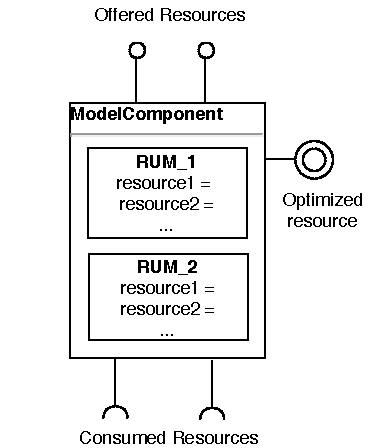
\includegraphics[width=0.5\linewidth]{resources/img/component.pdf}
  \caption{Notation of an RDM component with RUM's}
  \label{fig:component}
\end{figure}
\begin{figure}
\begingroup\centering
  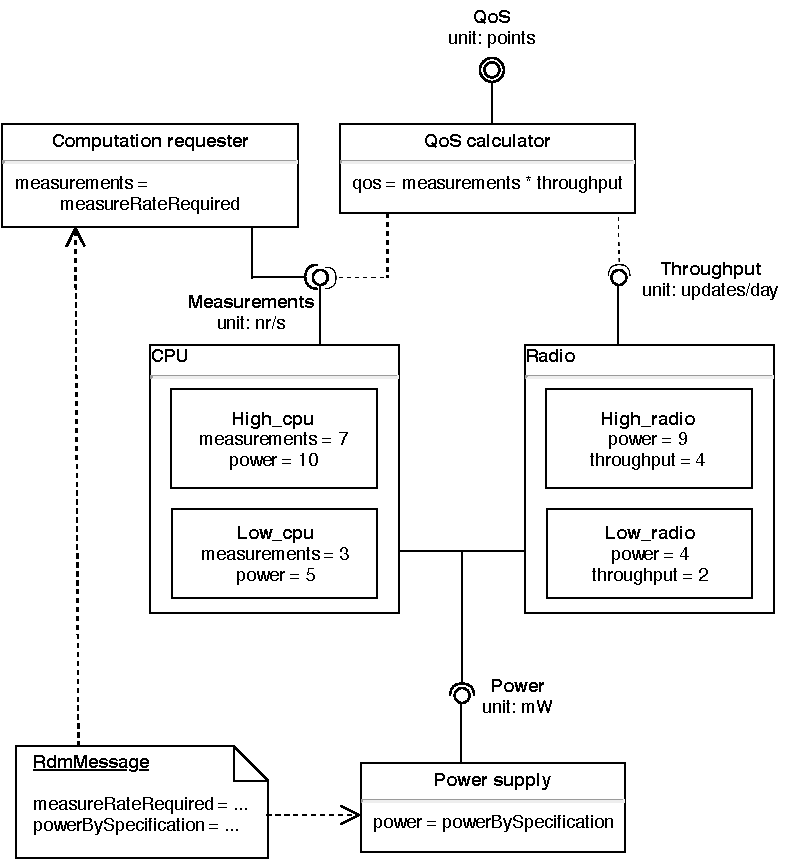
\includegraphics[width=\linewidth]{resources/img/rdm_cpu_radio.pdf}\endgroup \\ \\
  \noindent Constraints: \\
$c_1: cycles_{clock} >= cycles_{CPU}$ \\
$c_2: power_{power\_source} >= power_{CPU}+power_{Radio} $ \\ \\
\noindent Optimize:\\$max(QoS)$
\caption{Example instatiation of the RDM meta-model with a CPU and a radio}
  \label{fig:rdm_cpu_radio}
\end{figure}

%TODO insert pics
\subsubsection{Resource}
A resource is an entity describing a parameter of a system. This can be a measured parameter (e.g. battery capacity left or throughput), but can also describe a derived parameter (e.g. service time left). Each resource is identified by it's name and has a unit associated with it. By aggegating the ResourceInterfaces of a resource the amount of the resource produced and consumed can be collected and analysed.

\subsubsection{Component}
Any entity producing, consuming and converting a resource is represented by a component. A component can therefore be a physical entity such as a radio module or a battery or a hypothetical entity such as a QoS calculator executing a heuristic function. A component [contains] a ResourceFunction of each Resource it is connected to.
A [special] case of the Component is the ModelComponent. This class inherits all functionality of the ordinary Component, but its ResourceFunctions are extracted from one of its RUM's. Each RUM describes the parameters during one mode of operation of the components. This allows runtime analysis of variable behaviour as effect of different functionalities.

\subsubsection{ResourceInterface}
Resources and components are connected through resource interfaces. A ResourceInterface can be one of three types:
\begin{description}
\item[Offer] Indicating that the component produces an amount of the resource,
\item[Consume] Indicating that the component consumes an amount of the resource,
\item[Calculate] Special consume relation. This connection supplies 100\% of the offered resource, without formally consuming any amount. This relation is used to further calculate with the offered value, without it impacting the constraints of the resource. For example a QoS indicator that is ``consumed'' by a general QoS calculation.
\end{description}
Each interface has a value specifying the amount of the resource produced or consumed by the component. This value is repeatedly set and evaluated at runtime by executing a ResourceFunction.

\subsubsection{ResourceFunction}
The value of a ResourceInterface is determined by a ResourceFunction. This function constist of a function that takes a double array as argument and with a double as result, and an array of resource identifiers to fill the input array respectively. ResourseInterfaces can [compactly] be instantiated using lambda expressions and varargs. E.g.:
\begin{lstlisting}[language=java, frame=single, numbers=left, tabsize=4, basicstyle=\small]
ResourceFunction totalServiceTime = new ResourceFunction(
	(x)->x[0]+x[1], yearsServed, yearsLeft
);
\end{lstlisting}

To model the [gewenste] behaviour of the model we introduce a set of \textbf{Requirements} and an \textbf{Optimizer}.
\subsubsection{Requirement}
A resource can have any number of Requirements function as constraints that limit the possible values of [variation] of that resource. The standard built-in requirement for every resource is the \emph{OfferConsumeGTE} requirement which enforces that the amount produced needs to be greater or equal than the amount consumed. Additional requirements \emph{OfferConsumeEQ} and \emph{RangeRequirment} are supplied that respectively require the exact amount offered to be consumed and the amount offered or consumed to be within certain bounds. Finally the abstract class Requirement can be extended by a developer to specify any tailored requirement.
\subsubsection{Optimizer}
To [assertain] the heuristic [grade] of a RDM with a [gevulde] RUM configuration we introduce the Optimizer. The Optimizer is an extended class of Resource of which exaclty one must exist in an RDM. The optimizer takes the evaluated offered amount of the Resource and calculates a score. This score is a value on a comparative scale of which a higher value entails a more optimal solution. Supplied are the \emph{MinMaxOptimizer} which evaluates that the amount offered must have a minimal or maximal (specifiable) value and the \emph{ApproxOptimizer} which evaluates that the resource must have an amount offered as close to a specified value as possible. However, custom implementations of the Optimizer can again be made by developers.

\subsubsection{RdmMessage}
Finally, to supply the model with the state of the system under investigation, we pose the RdmMessage. The RdmMessage is provisioned using values measured from the system and injected in the model, after which the appropriate resource values are evaluated accordingly. Technically, a simple mapping from a resource name to a measured value value would do for this purpose, but this mapping is wrapped in an object to support future [expansions] of the object.

\subsection{Solving the model}
With the model well-esteblished, we can now try and solve the model. From requirement \ref{r:solvable} we find the goal of solving the model is to find a composition of RUM's such that:
\begin{enumerate}
\item each ModelComponent has exaclty one RUM associated with it,
\item all resource constraints are satisfied, and
\item the optimizer function of the optimized resource has the highest value.
\end{enumerate}
The first and second requirement implies constraint solvers as an applicable technology[. Since] they are effective in finding a valid solution for a constraint decision problem. However, the third requirement [implies] that we do not want to find any valid solution, but the optimal valid solution. In order to do that we need to consider \emph{every} valid solution to the problem and compare how they compare [heuristicly]. This entails a [brute force] search approach through the entire search[-]space of RUM compositions. We can however use constraint solver [paradigms] to preventively reduce the search space as we search through it.

The way we do this is by employing backtrack search. In a simple brute force search we would calculate all RUM compositions and for each composition we provision the full model and evaluate it. Instead we will iteratively select a component and one of its models. We will then not provision the entire model, but inject the selected model in the chosen ModelComponent. Consequently we calculate only those variables we can resolve with the information currently represented by the model. We then evaluate the resource constraints. Given an incomplete model any constraint can have one of three statuses:
\begin{itemize}
\item satisfaction,
\item failure, or
\item uncertain
\end{itemize}
for every consequent assingment of unprovisioned components.

If a constraint evaluates to \emph{satisfied} it will be pruned and not [evaluated] in the remainder of this [branch] of the search [tree], since we know it will always succeed. If a constraint is \emph{uncertain} we keep it, since we do not know its [state] for each and every future [state]. If even a single constraint \emph{fails} we know the remainder of this branch of the search tree will never be valid. Therefore we backtrack through the tree by partially rolling back model assignment. We then select a different model for the same component or a different component entirely and repeat the algorithm [ref to algorithm]. This way we do not re-evaluate constraints we already know the state of and do not [visit] paths we know will not satisfy the constraints. Given that we encounter unsatisfactory options early in the tree, this will eliminate large [parts] of the search tree. An example of this algorithm on the example posed in Figure \ref{fig:rdm_cpu_radio} is given in Figure \ref{fig:search_cpu_radio}. This application illustrates that using this algorithm, we eliminate a significant portion of the search tree. This is due to early constraint failure detection in the \emph{CPU=high\_cpu} banch of the tree.
\begin{figure}
%\documentclass[11pt,a4paper]{article}
%\usepackage{qtree}
%\begin{document}
\hrule
\vspace{10px}
\Tree [. {CPU=low\_cpu\\c_2 \hspace{1px} is invalid\\backtrack} [.{CPU=high\_cpu\\c_2 \hspace{1px} is valid\\prune c_2} {Radio=high\_radio\\c1 \vspace{1px} is invalid\\backtrack} [.{Radio=low\_radio\\c_1 \vspace{1px} is valid\\prune c_1} {valid composition found\\calculate optimizer score} ] ] ] \\

\noindent Legend: \\
\emph{Assignment\\Observation\\Action\\}
\hrule
%\end{document}
\label{fig:search_cpu_radio}
\caption{Application of backtrack search on RDM of Figure \ref{fig:rdm_cpu_radio}}
\end{figure}

\section{Discussion/evaluation}
why no state machine (rum\_ basis\_ 2, rum\_ basis\_ 89) To much calculation, repeatedly
	state machines are usefull for developing rpm's
(dis)advantages van explicit model

%\subsection{discussion}
%always possible to convert state to optimizable (hypothetical) heuristic resource [search def:heuristic]
%short vs long term
%	solved by explicitly focussing on long term. By choice, long rtt and long lifetime.
%	allows collapsing states to single state (single variable)
%	guarentees solvability
%measure vs derive
%	- every internal resource needs to be calculable from only eventual external, measurable resources %(transitive)
%	- no cyclical calculations
	





%What to represent
%	Components, calculators
%	resources
%		requirements
%		optimizable
%	resource distribution
%What inputs
%What outputs
%what actions





\chapter{Design method}
\section{Adaptation}
Application of the Design Cycle to these design artefacts
\section{Cycles architecture}
\section{Cycles RUM}

\newcommand{\nedapidsystems}{\nedapidsystemsnospace\space}
\newcommand{\idsystems}{\idsystemsnospace\space}
\newcommand{\nedap}{\nedapnospace\space}
\newcommand{\ublox}{\ubloxnospace\space}
\newcommand{\sensit}{\sensitnospace\space}
\newcommand{\nedapidsystemsnospace}{\nedap\space\idsystems}
\newcommand{\idsystemsnospace}{Identification Systems}
\newcommand{\nedapnospace}{Nedap}
\newcommand{\ubloxnospace}{u-blox}
\newcommand{\sensitnospace}{SENSIT}
\chapter{Proof-of-concept validation by case study}
\label{ch:validation}
This chapter will attempt to validate the applicability of the platform to the field of LPWA QoS monitoring and management. This will be performed by designing and developing a prototype monitoring application, based on the proposed platform. This will not be performed on the afore-used hypothetical example from section \ref{sec:example_case}. Instead, it will be performed on a commercial car parking application sensor application. 

Firstly, some background will be given on the sensor application to be monitored. Next, the goals, claims and methodology of the study will be declared. With the goal and means stated, the experiment will be performed by realizing a prototype monitoring application. As the actual implementation details are auxiliary, they will not be examined in detail. However, the implementation will be described superficially to contextualize the validation efforts. After implementation, the results of the validation study will be presented and their implications deliberated. This chapter will be concluded with a discussion on the results, conclusions and limitations of the study.
\section{Context of the case study}
\subsection{Background}
\label{sec:sensit}
The case the development platform will be applied to is to the \nedapidsystems smart parking application: \sensitnospace. \nedap\cite{web:nedap} is a Dutch company based in the city of Groenlo. They produce hardware-software integrated products for a plethora of industries, such as retail, health-care and smart city management. The department \idsystems\cite{web:idsystems} focusses on the latter category. They develop solutions for detection, identification and physical access management of people and vehicles. This is performed by employing a series of self-produced hardware products such as RFID tags, sensor devices and cameras, with accompanying software products and platforms. 
\subsubsection*{\sensit smart parking application}
The \sensit\cite{web:sensit} smart parking application is devised by \nedapidsystems to monitor parking lots and garages. It employ a huge amount (up to thousands per location) of affordable LPWA sensor nodes. Each individual parking spot is equipped with one of these sensors to determine its occupation. To determine changes in occupation, each sensor is equipped with an infra-red and magnetic induction sensor. Should a change in occupation be detected, a message containing the measured sensor deltas is sent to the back-end application. This granular approach to smart parking allows the \sensit application to monitor and visualise the occupation of individual parking spaces in a lot, garage or even across cities.

In order to communicate with the back-end the sensors employ wireless technology. Previously, the sensors were connected to sinks using a proprietary network of relay nodes. However, the recent proliferation of large-scale cellular IoT networks has caused \nedap to shift towards these technologies. This allows large numbers of sensors to a single cell tower, without the need of deploying and managing a network of relay nodes for new sensor deployments. Additionally, the efforts of managing and maintaining the network are outsourced to professional operators. To connect the sensors to the internet the \emph{Narrow-band Internet of Things} technology was determined to be most suitable. New \sensit sensors are therefore equipped with \ublox\cite{web:ublox} NB-IoT radio modules to connect them to operated cell networks.

\subsection{Conceptualization of the monitoring application}
This section will describe and scope the context of the QoS monitoring application to be developed. First, the input for the application, as emitted by the WSN application under investigation, will be examined. Subsequently, the characteristics of the expected outcomes of the application to be prototyped will be discussed.

\subsubsection{Sensor data signature}
The sensor devices send a message with key performance indicator (KPI) data alongside every data message it sends. Alternatively, it will send one of these messages periodically if no data messages are sent for 12 hours. When computed universally, a message rate was determined of about 15 messages per sensor per day. However, a specific per sensor analysis yields a message rate of between 10 and 50 KPI information messages on average per day, with some outliers for more active sensors which can reach up to 250 messages per day on a regular basis.

The data sent by the sensor contains some typical networking data points, such as source IP address, source port, source device ID, message sequence number and a timestamp. Additionally, the message contains a hexadecimally encoded string describing the KPI's collected by the \ublox radio module. The data collected by the \ublox module contains mostly data points depicting the signalling functions of the radio module. Such KPI's include the signal-to-noise ratio (SNR), signal quality (RSSI), Extended Coverage Level (ECL) and more. Additionally, the KPI information includes some physical attributes of the radio module. Attributes such as the module's uptime, number of restarts and temperature

The ordinary data plus the \ublox KPI data are contained within 128 Bytes of data. Considering the messaging rate of a typical sensor yields an imposed per sensor footprint on bandwidth of $\pm$1--6 KiB/day for the majority of sensors with outliers of $\pm$KiB/day for extremely active sensors.

At this moment only a few nodes equipped with the NB-IoT technology have been deployed. Consequently, a large-scale test bed for the to be prototyped monitoring application does not exist. Therefore, a simulated sensor environment has been devised to test the prototype application for contemporary and near-future smart parking applications. This simulation is based on data signatures and values observed over a half year period emitted by the few nodes that have been deployed.

\subsubsection{QoS monitoring needs}
In collaboration with \nedap\idsystems a list of requirements for the outcomes of the prototype was compiled. These consequences are to be effected by the prototype application, based on input from (simulated) sensors. However, the actual implementation of the prototype is secondary to this chapter, since the primary goal is to evaluate choices made for the underlying development platform. Therefore, a comprehensive, formalized requirements document has not been included in this thesis. However, the features required of the monitoring application to be developed will be described shortly, in order to contextualize the implementation efforts of the prototype.

The consequences the application must effect are classified into three categories. The first of which is sensor feedback. This entails commands sent to sensors to alter its execution strategy, based on observations made in the monitoring application. This can be based on individual sensor data, historic sensor data or higher-level data snapshots (e.g. sink level). An example of such feedbacks are to decrease data rates to guarantee a predetermined minimum sensor lifetime or due to poor cell connectivity. This functionality is currently not present in the \nedap sensors, but is intended in the future. Therefore, it will be implemented into the simulation environment to test the command \& control capabilities of the platform.

The second type of effect to be caused by the application is instant alerting. The primary use case for this kind of consequence is when physical maintenance is imminently required in the application or its network. Detectable causes of when this might be warranted have been deliberated with \idsystems and examples include:
\begin{itemize}
\nospace
\item a long term drop in coverage level which might indicate permanent obstruction of signal
\item extremely high temperature readings indicating an electrical malfunction
\item unusually long periods of inactivity or, conversely, extreme data bursts indicate a rouge node not executing according to a valid strategy.
\item calculations estimating node lifetime determining a node needs replacing.
\end{itemize}

The last type of consequence is reporting. The goal of this is to inform technicians, managers or clients on the general operation of the WSN application. This comprises two types of reporting. The first is \emph{periodical reporting}. Periodical reporting will primarily focus on business goals such as long term performance metrics, compliance to service level agreements of both service providers and clients, and prospected short-term maintenance efforts and costs. The other type of reporting is \emph{real-time reporting}. This is useful to technicians monitoring the performance of an application during its runtime. Use cases include monitoring the number of incoming events, latencies of sensor devices and sinks, environmental conditions (such as weather and temperature) and which sensor strategies currently are deployed. Notice that the real-time aspect of this type of reporting does not require events to be reported instantaneously since for such statistics a per second or minute update suffices.

%\section{Structure of the validation study}
%With the application, case and its context clear, the focus will be turned to detailing the validation study. Before executing our validation study, this section will first depict the taken process. We will begin by clearly stating the claims we aim to confirm and the bounds of our scope. Following that we will describe the intended method of testing those claims specifically by detailing the quantified criteria the platform implementation process must adhere to. We must note that these criteria will only cover the scope of the validation study, not the functional requirements of the implementation for the case. As mentioned before, though important for the outcome of the product for the company, for this validation study these requirements are ancillary.

%With the goals clearly stated, parametrized and quantified, we will design and implement a prototype monitoring application built upon the developed software platform, tailored to the QoS monitoring needs of \idsystems. As mentioned before the actual implementation details are secondary for validation purposes of this chapter. Therefore we will only touch upon it shortly without going into great detail. We will however give a short summary of the developed prototype to provide a context to the validation efforts. During and after the development process we will measure the relevant parameters required to evaluate the determined validation criteria. To conclude the investigative implementation, we will attempt to adapt the constructed application to a few hypothetical extension scenarios in order to explore the adaptability of the provided platform.

%We will conclude this chapter by stating, analysing and deliberating the results obtained by measuring and observing the development process. These results will be compared with the priorly determined criteria of the study. If these criteria are met, this will validate the claims they are meant to affirm. We will finish by discussing the process and results in order to deliberate the limitations and lessons learned regarding the proposed development platform.
	
%\section{Criteria of the Case Study}
\section{Method}
\label{sec:val:method}
This section will detail the approach taken for this preliminary validation study. First, the general approach of the study will be listed. After which, the claims to be examined will be detailed. The section will conclude with a short discussion on the scope and bounds of the study.
\subsection{General approach} 
In order to ascertain whether the level of abstraction of the platform can facilitate the needs of the intended monitoring application for \sensitnospace, a prototype implementation will be designed and constructed. The expected outcome is an instantiation of the platform that serves the QoS processing needs of \idsystemsnospace. 

The possible existence of such an instantiation demonstrates that (at least for this use case) the level of abstraction is low enough to expose the full functionality that is required  (\textbf{applicability}). In order to validate that the level of abstraction is low enough, but not too low (\textbf{usability}), the program instructions required for the platform instantiation will be considered. These required instructions should not be more then the instructions required for a hypothetical monolithic implementation, supposing the level of abstraction is not too high (applicability claim). Finally, the \textbf{adaptability} of the platform and its instantiations will be evaluated by introducing some minor changes to the features and requirements of the monitoring application. It will then be hypothesized what the consequent changes to the platform implementation are. Should the appropriate level of abstraction have been chosen, it should prove uncumbersome to adapt the topology to these novel conditions.

From a business perspective, the most interesting parameter to express these these efforts would be the time required to develop. However, this parameter is extremely subjective as it heavily depends on the level of skill of the developer and its familiarity with the technology. Therefore, effort will primarily be measured by the code required, expressed in number of instructions required to construct a monitoring application built by adoptation of the platform.
%TODO voor presentatie: goldylocks area.

\subsection{Claims}
\label{sec:claims}
The cardinal claim investigated is that the appropriate level of abstraction was chosen in the design of the development platform. This entails that the provided collection of components can be adapted to suit a plethora of purposes and target applications. Conversely, the level of abstraction is not that low-level that implementation requires unnecessarily large development efforts because basic procedures require repeated implementation. This claim mirrors research question \ref{rq:abstraction}, which asks ``What is the appropriate level of abstraction for a WSN monitoring platform [...]''. This claim is explicated into three sub-claims.

\subsubsection{Applicability}
Intuitively, the first criterium regarding the level of abstraction is that the platform features a level of abstraction low enough to facilitate the implementation of the monitoring application for \sensitnospace. I.e. the platform's abstraction does not obfuscate key functionalities which would require reimplementation of formerly present features. This seems an obvious and trivial demand, but without stating it, any subsequent criterium is pointless. More formally, the platform should enable an instantiation which enables iterative enrichment and aggregation of information. At multiple stages of the consequential iteration the application should be able to generate outputs such as alerts and reports for auxiliary processes and systems.

\subsubsection{Usability}
The second criterium to be validated is that the level of abstraction is not too low. Though the platform should enable an instantiation according to the needs of \nedap\idsystemsnospace, it should do so with minimal development effort. A level of abstraction that is too low requires application developers to repeatedly implement functionality that, due to their frequent nature, should have been provided by the platform itself. This criterium seems similar to the first, but the metrics determining their attainment are measured differently. Therefore, they will be regarded as two separate claims.

These development efforts will be expressed in the number of code instructions required to realize the implementation. Since an absolute benchmark was difficult to ascertain, the upper bound of permissible number of code instructions is established relative to the amount of instructions necessary for a functionally similar monolithic implementation. Should a larger code-base be determined, this entails a level of abstraction that is too low and requires (repeated) implementation of procedures that should have been provided by the platform itself. For the construction of the topology it was chosen to allow at most 4 operations for every component in the platform topology. The criterium of 4 operations per component originates from an assertion made in Chapter \ref{ch:architecture}.

\subsubsection{Adapatability}
The final criterium employed to validate the appropriate level of abstraction is that the platform facilitates convenient adaptation of a realized platform implementation. This validation will be performed by introducing or changing a minor feature (e.g. new input type, altered reporting requirement). Should the appropriate level of abstraction have been chosen, it should prove uncumbersome to adapt the topology to these novel conditions. For the adaptability of the application provided by the platform, it was determined that minor new features and requirements should require not more than
\begin{itemize}
\nospace
\item a localized rearrangement of the model/topology, and
\item introduction or major change of at most two components.
\end{itemize}
For all cases, small changes are allowed to the components interfacing with the altered component(s) in order to produce or consume information supplied to or emitted by the altered interface. Additionally, very minor, consistent changes are allowed to be made to other components. The reason for this is that often a change or introduction of a data point requires that data point to be propagated throughout the topology.

The rationale for these allowances is that the modularization provided by the platform should prevent entanglement of concerns and therefore minor changes should cause localized effects. There is however a possibility that (especially new features) require a change in several components since its the functionality was not previously present. Therefore, minor consistent changes are allowed to those components in order to forward the new functionality. Finally, the reason for the allowance of a major change in two components is that often computation and analysis of a data point is separated into distinct components due to separation of concerns. Therefore, a changed requirement will often require a change in both components.

%To recap, we validate the main claim by three sub-claims that are summarized as applicability, usability and adaptability. For the remainder of this chapter these three claims will be addressed using these headings. In full these claims read:
%\begin{description}[style=nextline]
%\nospace
%\item[Applicability] The platform's level of abstraction is low enough to suit a large number of applications,
%\item[Usability] The platform's level of abstraction is high enough that the framework prevents repeated implementation of common procedures, and
%\item[Adaptability] The platform facilitates effortless adaptation of an instantiated application.
%\end{description}
%Altogether, these claims culminate in the main claim that the appropriate level of abstraction has been chosen.

\subsection{Bounds}
Before executing the validation study, the bounds and limitations of this validation study will need to be considered. The first glaring limitation of this study is that it is extremely limited in scope. The platform will only be implemented for a specific WSN application and this study will therefore not state the platform to be appropriate for the entire set of applications that was determined in Section \ref{sec:back:context} of the background chapter. Instead, this study will at most affirm the platform as a proof-of-concept for WSN application QoS monitoring.

The second limitation worthy of notion is that, aside from only regarding a single WSN application, it will also run on a simulation of that application. As mentioned before, this is because the NB-IoT-incorporated sensor devices of the \sensit application have only recently started deployment. As a consequence, a test bed of significant scale is presently not available. However, simulating a full future deployment of the application enables easy adaptation of the WSN application under investigation, in terms of both scale and functionality. This allows to not only test for intended regular behaviour but also for extreme and niche conditions. Additionally, the simulated environment allows for easy temporal manipulation, which enables the simulation to be accelerated, halted and repeated.

\section{Implementation of the WSN monitoring application}
\subsection{Design and Implementation}
In this section the design for the platform instantiation for \nedap\sensit will be detailed. First, a top-down look at the entire topology will be taken. After which the functionality of the individual components will be described shortly. Finally, the instantiation of the Resource Distribution Model used to compute the state of sensors will be illustrated.

\subsubsection{Application topology}
The designed topology is depicted in Figure \ref{fig:sensit_topology}. This figure shows the processing to be divided into three stages. In the first stage raw-information snapshots are enriched and normalized. In doing so it improves the information potential and accuracy of the data in the snapshot. The second stage concerns sensor level analysis and management. It calculates the state and resource consumption of the devices, and it includes some services that alert if a sensor exhibits abnormal behaviour or long term deviations of its ordinary parameter margins. The final stage concerns snapshot accumulation in order to extract high level information and adaptations. This stage diverges into three distinct accumulator paths. The top path performs accumulations of snapshots based on the sensor group ID. It reports on data rate violations (as agreed upon in SLA's) and recalculates the share of the data each sensor within a sensor group is allowed to consume. The middle execution path concerns the cells served by nodes. It alerts if a node switches cells more then an allowed amount during a period. The bottom accumulates all snapshots in order to report on the current state of the application as a whole.
%TODO check paths
\begin{sidewaysfigure}
\centering
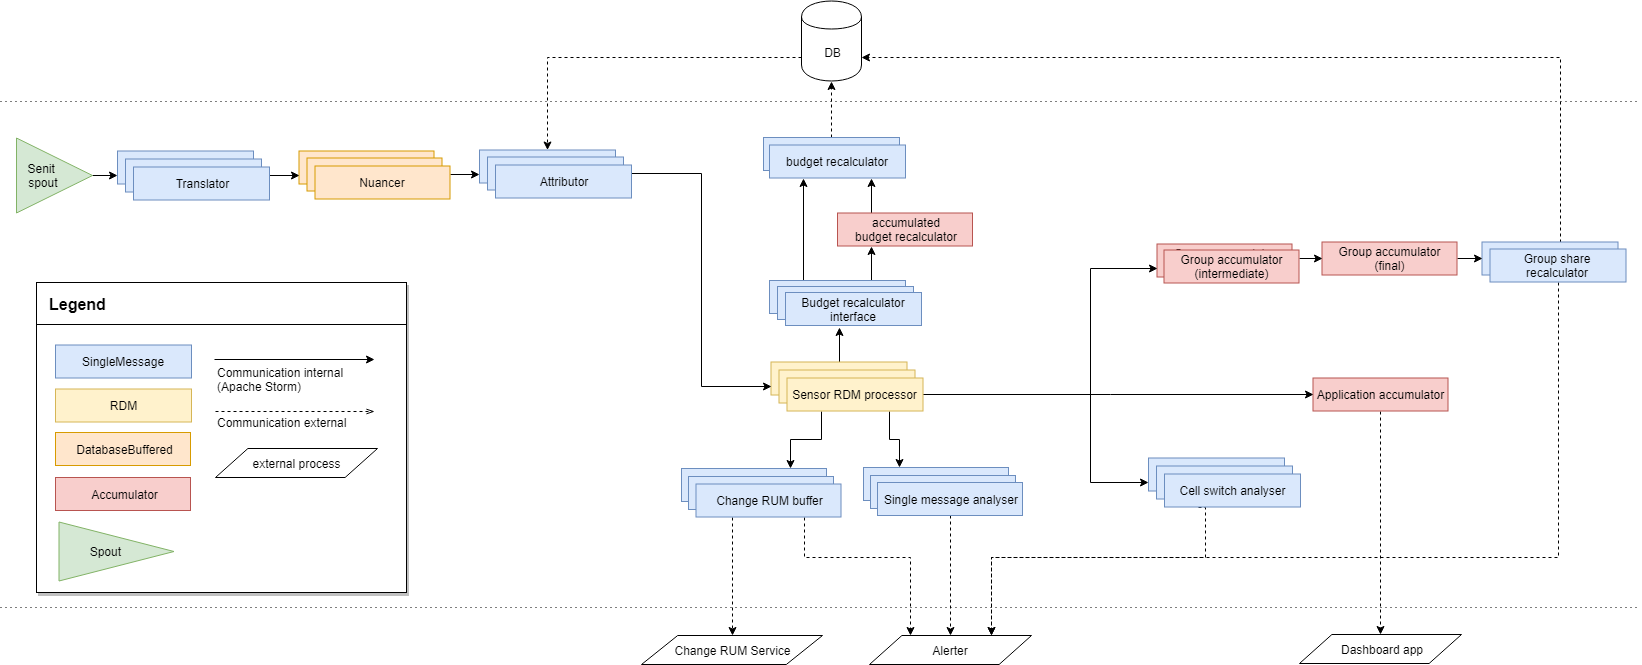
\includegraphics[width=1.15\textwidth]{resources/img/sensit_topology.png}
\caption{Topology of the monitoring application for the \nedap\idsystems\sensit WSN application}
\label{fig:sensit_topology}
\end{sidewaysfigure}

The description of the application topology will be concluded by shortly describing the functions of the individual components.
\begin{description}[style=nextline]
\nospace
\item[Sensit spout] Reads sensor snapshots from a Kafka channel and introduces them into the topology.
\item[Translator] Translates the sensor information from hexadecimal string to key-value pairs.
\item[Nuancer] Averages the data points received from a sensor to eliminate abnormalities. It does so by keeping a record of the last seen messages for each sensor node in an SQL database.
\item[Attributor] Enriches the snapshot with some data points not present in the sensor but known by  back-end services.
\item[Sensor RDM processor] Processes the enriched information from the snapshot and calculates the optimal operational device strategy.
\item[Switch strategy buffer] Buffers the switch strategy messages to prevent superfluous, erratic feedback to the sensors. Doesn't switch strategy on first report, only if a switch is requested over an extended period.
\item[Single message analyser] Calculates weather the sensor parameters, as calculated by the RDM processor, are within the allowable margins.
\item[Budget recalculator interface]If the message rate of a sensor is high enough will initiate an immediate budget recalculation. If message rate is low it is allowed to be accumulated over some time to reduce the number of database updates.
\item[Budget recalculator accumulator] Accumulates budget recalculation snapshots and prepares them for batch update.
\item[Budget recalculator] Executes (batch) budget recalculation.
\item[Group accumulator] Accumulates snapshots by sensor's group ID. Because this is performed on a weekly basis, this is performed two-stage as not to cause a large data build-up over time.
\item[Group share recalculator] Recalculates the share of the sensor group's resources each sensor is allowed to consume, based on the data used by each node over a one week period.
\item[Application accumulator] Accumulates the information emitted by the application in order to be presented on an application dashboard.
\item[Cell switch analyser] Analyses and reports if a node switches between cell towers more then is allowed.
\end{description}

A final remark on the application design is on the interfaces it provides. The application's inputs and outputs are received from and provided to Apache Kafka channels. This allows actual services to be easily swapped in and out with test services (even at runtime)

\subsubsection{Sensor Resource Distribution Model}
The Resource Distribution Model proposed in Chapter \ref{ch:rdm} is employed to model the state, behaviour and strategies of the sensor. The resulting model is depicted in Figure \ref{fig:sensit_rdm}. 

The model takes a few parameters based on the sensor state measurements, such as its current ECL and message rate, and its history, such as its runtime, data already used and messages already sent. Additionally, the model recieves some data points on the availability of resources such as the allowed number of messages during a time period (called the budget) and the allowed data usage for that sensor. The model then computes the runtime the sensor has left, current data and budget consumption and the future message rate. 

The variable behaviour of the \emph{MessageRateDeterminer} is curtailed by two constraints on the model. The first is that the \emph{budgetLeft} produced by the \emph{BudgetProvider} must exceed the amount that is consumed by the \emph{RemainingCalculator}, which is ultimately derived from the allowed message rate for the sensor device (\emph{messageRateFuture}). Similarly, the same holds for the \emph{dataLeft} produced by the \emph{DataProvider}. Should multiple RUM assignments evaluate as valid, the most optimal one is decided to be the one which provides the highest message rate.

%TODO reconfigure img to fit on page and be readable
%TODO resources non_cap_first, componets cap_first
\begin{figure}
\centering
\hrule
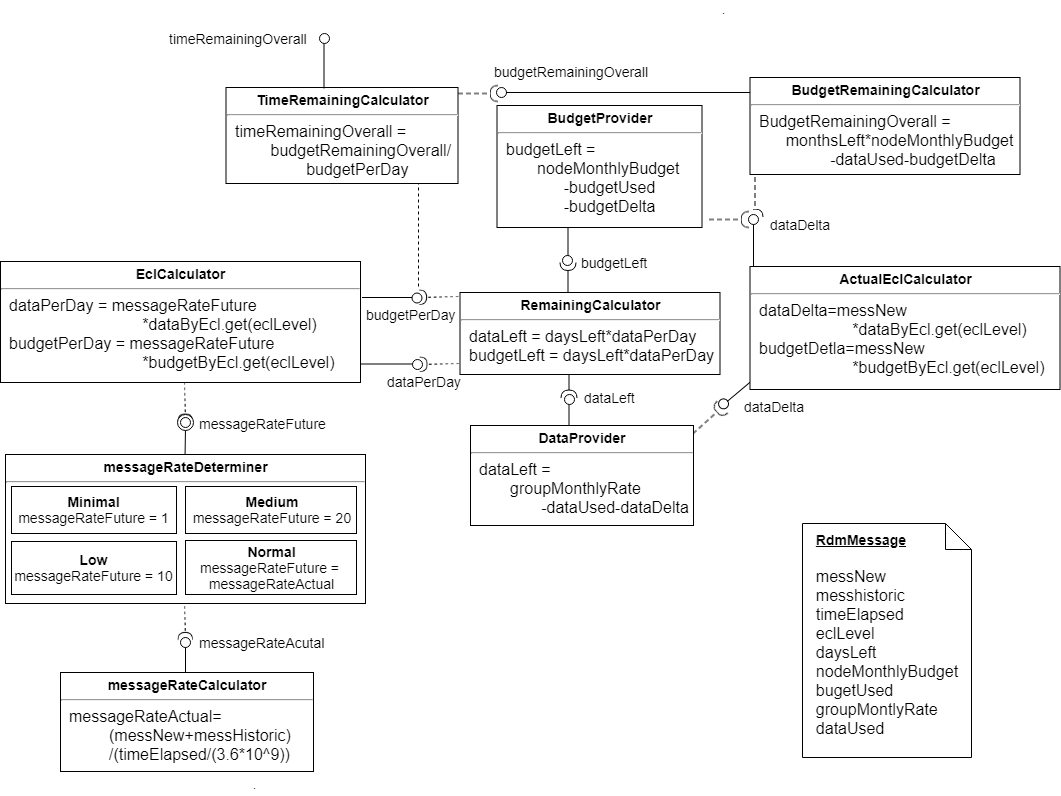
\includegraphics[width=\textwidth]{resources/img/sensit_rdm.png}
\hrule
\caption{Resource Distribution Model for a sensor in the \idsystems\sensit WSN application}
\label{fig:sensit_rdm}
\end{figure}

Preliminary experiments with resource consumption models have shown that, when a scarce resource is involved, a device will act differently in the beginning than in the end of its life-cycle. The reason for this is that in the beginning the models will instruct the device to operate on a strategy that will consume less resources then it is allowed on average. Then, when it has saved up enough of that resource, it is allowed to spend it on a strategy that consumes more than that average. To mitigate this effect it was decided to recalculate the available resources on a monthly basis. This way there is still such a cycle, but its period is far shorter and the effect will be much less and much more regular overall.

\subsection{Adapting the application}
This section will be concluded by deliberating some hypothetical adaptations in order to investigate the adaptability of the platform.

\subsubsection{Nuancer local}
The first change introduced is the constraint for the \emph{Nuancer} to not require a database connection. Reason for such a requirement could be to reduce latency or to eliminate capacity issues caused by employing an SQL database

This can be achieved by exchanging the current \emph{DatabaseBuffered} Nuancer implementation with a \emph{SingleMessageProcessor}. This processor keeps an in-memory cache of the last snapshots it has encountered, grouped by node and ordered by timestamp or sequence number. For each incoming snapshot the following sequence of actions is taken:
\begin{enumerate}
\nospace
\item determine node by ID,
\item add snapshot to the node's buffer,
\item prune out-of-scope snapshots from the buffer,
\item calculate average of remaining buffered snapshots, and
\item emit averaged snapshot
\end{enumerate}
This sequence of actions is similar to how the Nuancer operates in the current topology, but it eliminates the database connection in favour of a local buffer of snapshots. Unfortunately, by shifting to a local buffer the scaffolding provided by the \emph{BufferedComponent} can no longer be employed. The reason for this is that the component with local buffer (as currently implemented) operates on a single global buffer, instead of a buffer per node.

Finally, it must be noted that in requiring the snapshots to be cached locally, a large burden is forced upon the memory of the machine/container running the component. Should the application serve a large amount of nodes and snapshots are collected within a large window of interest, the data kept in-memory can rapidly reach large sizes. This can be alleviated by replicating this component to the point that individual memory requirements of workers are within manageable parameters. Alternatively, the memory issue can be evaded by persisting and reading snapshots to local files. This introduces some latency due to disk IO --- however far less than database communication does --- but can immensely reduce the number of records in the active cache at any time.

\subsubsection{New sensor data encoding}
As mentioned, the auxiliary performance data of the sensor is received as an encoded hexadecimal string. For this case, a new a new hypothetical type of sensor is introduced. This sensor equipped with a different radio module, which encodes its KPI data slightly differently. It is emphasized that the actual data collected and emitted by the sensors is not changed significantly. As this would entail a major change in how computations need to be performed. Though deliberated as a hypothetical, this case simulates a real future scenario. Since the aim is for a node lifetime of at least 10 years, it is very conceivable that wireless sensor technologies improve and change during that time frame. Since physical replacement of the large volumes of deployed nodes is unprofitable for both \nedap and its clients, this new technology should be supported in tandem with the old sensor types.

This change in the sensor environment can be accommodated by introducing a second \emph{Translator} component specifically intended for the new data format. This component is executed independently of --- and in parallel to --- the original Translator. How to ensure that a snapshot is processed by the correct translator, will depend on how the new data stream is supplied to the application. This hypothetical will consider the most complicated input option, where the old and the new style snapshots are emitted on a single input channel. An interface component is introduced to split the singular input stream into two. This component performs a superficial inspection of the snapshot and forwards it to the correct Storm channel based on some discerning feature (e.g. data format or type identifier). Though technically this inspection could be performed by the \emph{SensorSpout}, separation of concerns compels a separate component for this purpose. Ultimately, both translators uniformly emit their translated snapshots to a common Storm channel for further processing. The resulting partial topology is illustrated in Figure \ref{fig:update_encoding}

\begin{figure}
\centering
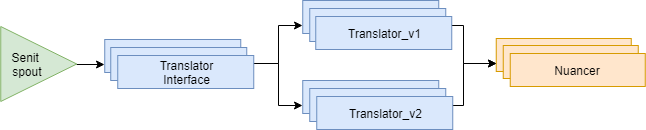
\includegraphics[width=\textwidth]{resources/img/update_encoding.png}
\caption{Updated partial topology for new data encoding}
\label{fig:update_encoding}
\end{figure}

\subsubsection{Alert on long-term ECL drop}
For the final case, the functionality of the application is extended by introducing a new outcome for the application. The added requirement is the detection of long term drop in ECL level. Such a drop could signify a (possibly alleviable) obstruction placed between the sensor and sensor sink (cell tower). Moreover, should several geographically related sensors report such a disruption, drastic actions cannot be ignored. In the topology this can easily be achieved by extending one of the existing components. 

Formally, the \emph{CellSwitchAnalyser} would be most suited for this purpose, since it is already historically aware due to retaining a list of cell towers per sensor. Though the component would obviously require renaming. This functionality is provided by keeping a list of ECLs reported by each sensor node. When the sightings are inconsistent or do not feature a drop, the list is pruned. When the list's size surpasses a set threshold --- i.e. a consistent ECL drop has occurred --- an alert is sent to the alerter. This is easily implemented since the CellSwitchAnalyser already features alerting functionality. Finally, this change does not require changes to interfacing components, since the ECL level is already present in the snapshot emitted by the \emph{SensorRdmProcessor}.

\section{Results \& Evaluation}
\label{sec:resultseval}
The results of the study will be reported in accordance with the three sub-claims and discussed under their own three headings: applicability, development effort and adaptability.

\subsubsection{Applicability}
The sensor model was found to be adequate for modelling the behaviour of the \sensit sensors. The modular design proved very useful for expositioning the different resources and how they were interconnectively calculated and distributed. Unfortunately (for the purpose of this study), the sensor did not feature a large variety of resource metrics specifying its configurable behaviour and therefore the model only featured one configurable component. Additionally, after accumulation of the application-level parameters by the \emph{ApplicationAccumulator} the accumulated parameters needed no further transformations and the WSN application did not feature application-level configuration needs. Therefore, the Resource Distribution Model was only employed on the sensor-level.

The result of the applicability investigation with regard to the distributed topology is that the platform suffices as development platform for the purposes of \nedap\idsystemsnospace. The provided building blocks enable the implementation of a functional application and provide functional abstraction of the specifics of the underlying technologies. During implementation of the application it was noted however that the platform does not provide an efficient way of buffering and processing snapshots grouped per node, cell tower, etc. This functionality could easily be provided by implementing the \emph{BufferedProcessor} with multiple buffers. A mapper function introduced to the processor will then determine which buffer a snapshot will be added into. The existing filter, sort and execution methods will then be performed on these buckets individually, providing a mechanism of grouped computations.

However, such functionality currently is not present, this absences was easily compensated for and was found to be only a minor inconvenience. This issue singularly was not sufficient to invalidate the applicability criterium. Therefore, it is stated that the applicability criterium holds.

\subsubsection{Usability}
Specifying the sensor model and application topology could be performed within the set parameters. As claimed, each component requires but four actions to be introduced to the topology. These actions are:
\begin{enumerate}
\nospace
\item create component, 
\item declare component, 
\item subscribe consumer channels, and 
\item declare output channels. 
\end{enumerate}
However, the internal code of the topology components, which actually performs the calculations and computations, required more code that a monolithic alternative would. While the actual number of lines of code was only a little higher than then its monolithic counterpart, the computations and transformations performed on those lines was far more then would be necessary in a monolithic application. These discrepancies will be deliberated on further in Section \ref{sec:resultseval}.

This was also reflected in the time required to develop this prototype. It was initially expected that the instantiation could be constructed within 40 man-hours. However, this eventually took twice as many hours. Of that time about 15\% was spent designing, 35\% developing and 50\% debugging the application\footnote{All hours spent after fully constructing and first execution of the application are pooled into the latter category}. The breakdown of the time spent yields that it took an enormous amount of time to debug and adapt the components after its original design and implementation. The chief reason for this was found to be the loose coupling between components. The components are completely disjoint and the snapshot variables they share require custom serialization between components and are accessed with string identifiers. This entails that it is excessively easy to implement a component pair with mismatched coupling. This is since inappropriate variable access due to misspelled identifiers can occur very easily and is not detected by code checkers and compilers of conventional programming tools. Subsequently, when the variable is accessed successfully, the value often requires deserializing into the correct primitive or object type. This again introduces a possible point of failure due to misparsing and miscasting, since the compiler cannot detect the actual object type before executing the application.

The introduction of snapshot struct objects (POJOs) is proposed to alleviate both above mentioned problems. These objects contain the variables of the snapshots passed between components. However, in contrast to loosely coupled key-value bindings, these bindings are explicitly defined in both type and identifier. They can therefore easily be serialized and deserialized by common serialization mechanisms. This would alleviate the need for developers to continually specify custom serialization. By providing direct access to the correctly parsed variables in the snapshots it will reduce the code base by a huge amount. Additionally, by providing a mechanism to directly access the properly parsed variables, the number of possible instances where mismatching, misparsing and miscasting can occur is reduced. Thereby eliminating several points of possible failure which have proved problematic. Combined, this increased traceability and automated (de)serialization should have a noticeable, positive effect on the amount of required code. Consequently, it will reduce the time spent debugging and reworking the application and thus the development time as a whole.

To illustrate this benefit, two simplified code snippets from the \emph{SensorNuancer} are presented. One which does not employ structs (Listing \ref{list:nuancer_without_structs}) and one which does (Listing \ref{list:nuancer_with_structs}). From these examples it is clearly observable that by employing well-defined, serializable structs, the instructions required are reduced. Additionally, it reduces the chance of mismatching variable identifiers by eliminating string bindings.

%TODO placement
%TODO line numbers
\begin{scriptsize}
\begin{minipage}{\textwidth}
\begin{lstlisting}[
language=java, 
caption={Simplified fragment of \emph{SensorNuancer} without struct objects}, 
label={list:nuancer_without_structs}, 
escapeinside={(*}{*)}, 
captionpos=b,
numbers=left,
tabsize=4
]
public void runForMessagesHistoric(LinkedList<IOMessage> history) {
	Map<String, String> args = new HashMap<>();
	long first = Long.parseLong(
		history.getFirst().getVars().get("TIMESTAMP"));
	long last = Long.parseLong(
		history.getLast().getVars().get("TIMESTAMP"));
			
	List<Integer> ecls = new LinkedList<>();
	for(IOMessage m : history){
		ecls.add(Integer.parseInt(m.getVars().get("ECL_LOCAL"));		
	}
	int normalizedEcl = normalizeEcl(ecls);
			
	args.put("MILLIS_ELAPSED", Long.toString(last-first));
	args.put("ECL_LOCAL", history.getLast().getVars().get("ECL_LOCAL"));
	args.put("ECL", Integer.toString(normalizedEcl));
	publish("SENSOR_NORMALIZED", new IOMessage(args));		
}
\end{lstlisting}
\end{minipage}
\end{scriptsize}
\begin{scriptsize}
\begin{minipage}{\textwidth}
\begin{lstlisting}[
language=java, 
caption={Simplified fragment of \emph{SensorNuancer} with struct objects}, 
label={list:nuancer_with_structs}, 
escapeinside={(*}{*)}, 
captionpos=b,
numbers=left,
tabsize=4
]	
public void runForMessagesHistoric(LinkedList<NuancerInStruct> history) {
	NuancerOutStruct output = new NuancerOutStruct();
	long first = history.getFirst().getTimestamp();
	long last = history.getLast().getTimestamp();
			
	List<Integer> ecls = new LinkedList<>();
	for(NuancerInStrcut struct : history){
		ecls.add(struct.getEclLocal());
	}
	int normalizedEcl = normalizeEcl(ecls);		
			
	output.setMillisElapsed(last-first);
	output.setEclLocal(history.getLast().getEclLocal());
	output.setEcl(normalizedEcl);				
	publish("SENSOR_NORMALIZED", output);	
}
\end{lstlisting}
\end{minipage}
\end{scriptsize}

Finally, it was noted that after initially specifying the topology and models, reworking them proved to be frustrating. The difficulty was mainly in locating the instantiation and declaration of a component in the code that builds the topology. The reason for this is that it constantly requires a developer to transition from a two-dimensional graphic image of the model or topology to builder code which is one-dimensional (lines of code). This mental transition can be avoided by eventually developing graphic development tools that allows a developer to conceive a topology by drawing a graphical model of components and resources. The appropriate computational code can then later be introduced into the components. By doing so, a developer would only need to concern themselves with one depiction of the topology instead of two.

\subsubsection{Adaptability}
Finally, the necessary adaptations to the existing application for each hypothetical case are summarized in Table \ref{table:adaptations}. The table depicts that all three scenarios conform to the set criteria. All minor changes to the requirements context were incorporable with the existing application by introducing or changing at most two components. Additionally, the adaptations required either no changes to the topology or only small, localized changes. Incidentally, these scenarios required no changes to the components interfacing with the changed or introduced components.

\begin{table}
\centering
\begin{tabular}{|l||c|c||c|c|} \hline
Summary				& \multicolumn{2}{c||}{Components}		& \multicolumn{2}{c|}{Topology changes} \\ 
					& new 	& changed 	& none 		& only local  \\ \hline 
Nuancer local		& 0		& 1			&			& \cmark \\ \hline
New sensor encoding	& 2		& 0			& 			& \cmark \\ \hline
Alert ECL drop		& 0		& 1			& \cmark	&		 \\ \hline
\end{tabular}
\caption{changes required per adaptation scenario}
\label{table:adaptations}
\end{table}

%Applicability
%	goed, mist mapped-buffer
%2x zolang als gepland
%	tracability difficult
%	disjunction 2d model, 1d coding
%	debug first run duurt lang want string-bindings en string serialized
%	part testing is goed (dump result/intermediate)
%	solved by structs
%Meer code dan gepland (bijna 2x zovel)
%	building models en topology wel goed
%	(de)serializing
%	solved by structs
%[todo:timing/scalability]
%\section{Evaluation}
%\label{sec:eval}
%This section will evaluate the obtained results and compare them to the criteria set out in section \ref{sec:claims}. The criteria will be deliberated in the same order as the results in the previous section were.

%\subsubsection{Applicability}
%As stated, the building blocks provided by the platform allowed for a sufficient implementation of the intended monitoring application. However, it was discovered that, though possibly useful, the platform did not provide an efficient template to buffer snapshots grouped by a certain snapshot parameter.  This component could easily be provided by introducing a mapper function to the \emph{BufferedProcessor} which will determine into which buffer a snapshot will be added to. The existing filter, sort and execution methods will then be performed on these buckets individually, providing a mechanism of grouped computations.

%However, such functionality currently is not present, this absences was easily avoided and was found to be only a minor inconvenience. Since this issue singularly was not sufficient to invalidate the applicability criterium, Criteria 1 is stated to hold.


%\subsubsection{Usability}
%As mentioned it took about 80 hours to construct an develop the prototype application. This is twice as many as was originally stated in the validation criterium (Criterium 4). 
%As mentioned in the results, though the code required to compose the resource models and application topology was contained within the specified parameters, the code required for the internals was found to be significantly more than a monolithic application would require. Therefore, it is yielded that \emph{usability} criterium was invalidated. The chief reason that the component internals required  more instructions as required in a monolith is the repeated serialization an deserialization of data into messages. Processing of each (group of) snapshot(s) is prepended with a few lines of code that extract, parse and cast each individual variable from the snapshot. After the component's processing is performed, a new snapshot is prepared with variables that again require its values to be serialized. When the computations of a component only amount to a few lines of code, this (de)serialization can quickly require more code than the actual computations do.

%This was also reflected in the time required to develop this prototype. It was initially expected that the instantiation could be constructed within 40 man-hours. However, this eventually took twice as many hours. Of that time about 15\% was spent designing, 35\% developing and 50\% debugging the application\footnote{All hours spent after fully constructing and first execution of the application are pooled into the latter category}. The breakdown of the time spent yields that it took an enormous amount of time to debug and adapt the components after its original design and implementation. The chief reason for this was found to be the loose coupling between components. The components are completely disjoint and the snapshot variables they share require custom serialization in between components and accessed with string identifiers. This entails that it is excessively easy to implement a broken component. This is since inappropriate variable access due to misspelled identifiers can occur very easily and is not detected by code checkers and compilers of conventional IDEs. Subsequently, when the variable is accessed successfully, the value often requires deserializing into the correct primitive or object type. This again introduces a possible point of failure due to misparsing and miscasting, since the compiler cannot detect the actual object type without executing the application.

%The introduction of snapshot struct objects (POJOs) is proposed to alleviate both the above mentioned problems. These objects contain the variables of the snapshots passed between components. However, in contrast to loosely coupled key-value bindings, these bindings are explicitly defined in both type and identifier. They can therefore easily be serialized and deserialized by common serialization mechanisms. This would alleviate the need for developers to continually specify custom serialization. By providing direct access to the correctly parsed variables in the snapshots it will reduce the code base by a huge amount. Additionally, by providing a mechanism to directly access the properly parsed variables, the number of possible instances where mismatching, misparsing and miscasting can occur is reduced. Thereby eliminating several points of possible failure which have proved problematic. Combined, this increased traceability and automated (de)serialization should have a noticeable, positive effect on the amount of required code and the time spent debugging and reworking the application, and thus the development time as a whole.

%To illustrate this benefit, two simplified code snippets from the \emph{SensorNuancer} are presented. One which does not employ structs (Listing \ref{list:nuancer_without_structs}) and one which does (Listing \ref{list:nuancer_with_structs}). From these examples it is clearly observable that by employing well-defined, serializable structs, the instructions required are reduced. Additionally, it reduces the chance of mismatching variable identifiers by eliminating string bindings.

%\begin{scriptsize}
\begin{minipage}{\textwidth}
\begin{lstlisting}[
language=java, 
caption={Simplified fragment of \emph{SensorNuancer} without struct objects}, 
label={list:nuancer_without_structs}, 
escapeinside={(*}{*)}, 
captionpos=b,
numbers=left,
tabsize=4
]
public void runForMessagesHistoric(LinkedList<IOMessage> history) {
	Map<String, String> args = new HashMap<>();
	long first = Long.parseLong(
		history.getFirst().getVars().get("TIMESTAMP"));
	long last = Long.parseLong(
		history.getLast().getVars().get("TIMESTAMP"));
			
	List<Integer> ecls = new LinkedList<>();
	for(IOMessage m : history){
		ecls.add(Integer.parseInt(m.getVars().get("ECL_LOCAL"));		
	}
	int normalizedEcl = normalizeEcl(ecls);
			
	args.put("MILLIS_ELAPSED", Long.toString(last-first));
	args.put("ECL_LOCAL", history.getLast().getVars().get("ECL_LOCAL"));
	args.put("ECL", Integer.toString(normalizedEcl));
	publish("SENSOR_NORMALIZED", new IOMessage(args));		
}
\end{lstlisting}
\end{minipage}
\end{scriptsize}
\begin{scriptsize}
\begin{minipage}{\textwidth}
\begin{lstlisting}[
language=java, 
caption={Simplified fragment of \emph{SensorNuancer} with struct objects}, 
label={list:nuancer_with_structs}, 
escapeinside={(*}{*)}, 
captionpos=b,
numbers=left,
tabsize=4
]	
public void runForMessagesHistoric(LinkedList<NuancerInStruct> history) {
	NuancerOutStruct output = new NuancerOutStruct();
	long first = history.getFirst().getTimestamp();
	long last = history.getLast().getTimestamp();
			
	List<Integer> ecls = new LinkedList<>();
	for(NuancerInStrcut struct : history){
		ecls.add(struct.getEclLocal());
	}
	int normalizedEcl = normalizeEcl(ecls);		
			
	output.setMillisElapsed(last-first);
	output.setEclLocal(history.getLast().getEclLocal());
	output.setEcl(normalizedEcl);				
	publish("SENSOR_NORMALIZED", output);	
}
\end{lstlisting}
\end{minipage}
\end{scriptsize}

%Finally, it was noted that after initially specifying the topology and models reworking them proved to be frustrating. The difficulty was mainly in locating the instantiation and declaration of a component in the code that builds the topology. The reason for this is that it constantly requires a developer to transition from a two-dimensional graphic image of the model or topology to builder code which is one-dimensional (top-to-bottom). This mental transition can be avoided by eventually developing  graphic development tools that allows a developer to conceive a topology by drawing a graphical model of components and resources. The appropriate computational code can then later be introduced into the components. By doing so a developer would only need to concern themselves with one depiction of the topology instead of two.

%\subsubsection{Adaptability}
%Table \ref{table:adaptations} depicts that all three scenarios conform to the set criteria. All minor changes to the requirements context were incorporable with the existing application by introducing or changing at most two components. Additionally, the adaptations require either no changes to the topology or only small, localized changes. Incidentally, these scenarios required no changes to the components interfacing with the changed or introduced components.

%applicability passd, with small notion
%devtime -> fail
%	tracability difficult
%	disjunction 2d model, 1d coding
%	debug first run duurt lang want string-bindings en string serialized
%	part testing is goed (dump result/intermediate)
%	solved by structs
%timing/scalability TODO
\section{Conclusion \& Discussion}
This chapter will be concluded by contemplating the outcomes. Firstly, the conclusions drawn from the performed study will be stated. Secondly, the validity of the study and therefore the conclusions drawn from it will be discussed. This chapter will be concluded by deliberating the limitations of this preliminary validation study.
\subsection{Conclusions}
The main conclusion to draw from this initial validation study is that it indicates the development platform to be a functional tool to develop a functional WSN monitoring application. The distributed application architecture provides a functional separation of concerns and the provided component scaffolding provides curtailment of most types of data streams and distributions. Secondly, the explicit Resource Distribution Model provides a useful exposition of how resources within a system are interconnected, calculated and utilized. Additionally, the explicit nature of the model allows unknown variables to be computed in accordance with the model's constraints and optimal behaviour.

This study has shown that, for the purpose of the \nedap\idsystems\sensit application, the monitoring solution can be constructed within the set parameters for required development effort, with the exception of the required implementation of component's internals. Additionally, the provided capability for separation of concern allows for rapid software evolution with respect to minor changes to the monitoring application's requirements or context. There are however some small deficiencies and issues to be solved in order to also make the platform more practicable

The first main issue to be resolved is the inclusion of functionality to buffer snapshots grouped by some parameter(s) of those snapshots. The second issue regards the inclusion of structs (POJOs) used to communicate between components. These structs can be automatically serialized and deserialized and they increase the traceability of data points between components. This will reduce the code and time required for development. It might be argued that these structs themselves will introduce new code to the application. However, these objects are easily generated by conventional code generators. This approach will therefore reduce the overall development effort required. As the components will no longer be disjunct, but coupled by these objects, it will reduce the time spent debugging the application significantly.

Secondly, the inclusion of a graphical model/topology editor will remove the disjoint between graphical design documents and actual implementation. This will further reduce the development effort as a developer is no longer required to transition constantly between two representations of the developed artefacts.

\subsection{Discussion}
To solidify the validity of this study, some contending issues must be addressed

\subsubsection{Representativeness of the \sensit application}
The first issue of which is the applicability of the study. For any assertion to be relevant to the field of LPWA WSN it must be demonstrated that the \sensit application is representative and conforms to the characteristics for LPWA WSN applications. Table \ref{table:LPWA-chars} lists the typical LPWA WSN characteristics, as reported by multiple sources \cite{lora_vs_sigfox_boek, lora_vs_sigfox_whitepaper, nbiot_vs_lora_vs_sigfox, lora_vs_sigfox, tmobile, nbiot}.

\begin{table}
\centering
\begin{tabular}{|l|l|}\hline
Characteristic & Value \\ \hline
Message payload & $<$256 Bytes	\\ \hline
data rate &	$\pm$1.6 KiB/day/node\footnotemark \\ \hline
node lifetime & $>$10 years \\ \hline
node costs & $<$5 USD \\ \hline
Network infrastructure & Star topology (cellular)	\\ \hline
\end{tabular}
\caption{Characteristics of typical LPWA WSN applications}
\label{table:LPWA-chars}
\end{table}

\footnotetext{Objective message/data rate bounds are difficult to obtain, since different technologies prioritize varying limiting factors (message rate, data rate, energy consumption, etc.)}

From the table summation and the application parameters stated in Section \ref{sec:sensit} it is conclude that the \sensit application conforms to the typical features of LPWA WSN applications. Intuitively, the node costs and lifetime, 5\$ and 10 years respectively, match the parameters typifying LPWA applications. Additionally, \sensit 's new NB-IoT network technology features the typical cellular star topology. More importantly, the LPWA data signatures encompass the data signatures featured by the \sensit application. The [100] Bytes per message are well contained within the typical maximum of 256 Bytes. Finally, supposing a message rate of 15 message per day and a payload of [100] Bytes per message yields a daily per sensor data rate of about 1.5 KiB. Though the actual daily message rate of a node can vary wildly, as do the general bounds for individual network technologies, the averaged rate conforms to the approximated per sensor data rate typical of LPWA WSN applications.

\subsubsection{Threat of over-abstraction}
As mentioned, the current state of the development platform features some deficiencies. Should these aforementioned deficiencies be absolved and the new functions provided, the level of abstraction is raised. Therefore, it must be ensured that the level of abstraction is not raised to the point that the applicability claim (sub-claim 1) is invalidated. For the inclusion of a \emph{MappedBufferedProcessor} this concern is trivial as it provides an abstraction but, as it is extends to the platform, it does not obfuscate any underlying functionality. In selecting or implementing a serialization mechanism, note should be taken that it can transform every innate or user-specified datatype. Provided this concern is considered, a higher level of abstraction is provided, but no functionality is lost. Finally, the to be included graphical modelling/development interface should allow definition, specification and interconnectivity between all components provided by the platform. To this end, it is urged that the graphical interface is included in the platform instead of developed alongside the platform as a separate project. Separate project development will inherently lead to the development of the graphical interface trailing the development main platform and possible diverging of goals and requirements. If curtailment of all the above mentioned concerns is guaranteed, the level of abstraction can be raised to an appropriate level while safeguarding the applicability claim.

\subsubsection{Developer skill level}
A final point of contention regarding the validity of this study is the subjectivity of the executor. The study was performed by a subject with full knowledge of the internals of the development platform. Though this allows for rapid development and exploration of the capabilities of the platform, it possibly undermines the conclusions made on required development effort. Reason for this is that the actual subject may be over-skilled with regard to a representative developer of a QoS monitoring application. Therefore, care must be taken that the general development effort is not underestimated. The likelihood of such an underestimation will be deliberated in this section.

Firstly,the construction of Resource Distribution Models will be deliberated. Though this study does not assert bold claims regarding the effort of constructing such models, the relative impact of a reduced skill level to the effort required can be predicted and discussed. Though a model instantiation may seem daunting, it is actually constructed using only a few concepts. A model consists of \emph{Resources} and \emph{Components} computing, consuming and producing these resources. Respectively, components are connected to resources by an interface of type \emph{Calculates}, \emph{Consumes} or \emph{Produces}. The only issue complicating this depiction is the \emph{ModelledComponent}, which contains multiple utilization models with a resource interface for each resource interfaced by the component. However, these interfaces are instantiated and act equal to the regular component-resource interfaces. Therefore, understanding of one carries over to the other. Finally, specifying the intended model may prove challenging to less familiar developers. This is due to the nature of the formula specification of resource interfaces. These formulas are very formalized to enable automated computation and evaluation of instantiations. These interface formulas take an array as input containing all input values required to compute its output. Consequently, a list of resource identifiers is provided to the function, specifying the resources to be inserted at each index of the input array. In doing so it provides a compact specification for these formulas. However, it also allows for construction of invalid, incalculable or semantically incorrect models. Therefore, clear and indubious instructions will be provided to guide future developers.

Finally, consequences to the application topology are considered. Firstly, the internals of the topology components are plain Java code. Therefore, the level of familiarity has a negligible effect to implementation of the internals. Secondly, the suggested introduction of a formalized and automated (de)serialization will only aid an uninformed developer, since it provides a clear handle to the implementer, obfuscating the cumbersome details of the underlying communication platform. Additionally, the construction of the application topology was concluded to be specifiable by four instructions per topology component. The skill level of the application developer/designer has no impact to this required number of instructions, since the provided \emph{TopologyBuilder} contains no actions aside these four instructions for a component: create component, declare component, subscribe to channels, declare as producer to channels

Finally, it is argued that an unskilled implementer will gain more from the platform then the acquainted subject which performed this study. This is asserted due to the limited number of component types that require understanding. The platform only features five different types of components, with at most two variations per component (e.g. distributed/local computation or database/local buffer). Additionally, the scaffolding provided will help developers in specifying more complicated components. For example the \emph{DatabaseBufferedComponent} requires implementations for abstracted methods that subsequently \emph{add to}, \emph{fetch} and \emph{filter} the buffer managed by the database. This sequence specification guides a developer in implementing the intended behaviour of the buffer. Therefore, it is argued that a less skilled developer will gain more benefit from the platform, relative to his/her skill level.

\subsection{Limitations and recommendations}
%TODO repeated execution (different applications) cements claims and boundries
Though this validation study demonstrates the platform to be a useful tool, it must be regarded as a proof-of-concept. This study only regarded one sensor application and therefore the results might be accidental and therefore the evidence provided by them is highly anecdotal. Though the preliminary results do indicate the platform to be a useful tool for WSN QoS monitoring, general statements are not allowed to be asserted unequivocally regarding the general applicability of this tool to the field of WSN applications. For such conclusions to be asserted, much more validation on a more varied base of applications is required.

A second shortcoming of this study is that the \sensit wireless sensor application did not feature the complex cases to fully explore the capabilities of the Resource Distribution Model. Previous chapters have claimed that the Resource Distribution Model should be applicable at multiple stages of information processing (e.g. sensor, per cell, entire application). However, as mentioned before, there was no case for post-accumulation processing or sensor configuration based on application-level parameters. Therefore, no RDM was employed in the latter stage of information processing. Therefore, the model is claimed to be applicable at sensor level for the \sensit application. In order to assert the model as a general solution, more research should be performed on sensor applications that do feature more complex application level processing or configuration.

Procedurally, this study also features a large limitation and therefore so do the conclusions drawn from it. The limitation to the study is that it was not designed as a blind study. As the application instantiation of the platform was developed by a developer with full knowledge the validation criteria and intimate knowledge of the internals of the development platform. In order to fully and objectively assert the conclusions of this study the experiment must be repeated more formally with impartial subjects. These subjects must be able to repeat the experiments process without knowledge of the parameters of the study, without familiarity of the platforms internals and only the provided documentation of the platform and its exposed APIs.

However, this eventual full-scale study should not be performed until the latter stages of platform development and validation. The reason for this is that it is far more resource-efficient to discover initial deficiencies and issues with small case studies, as performed in this chapter. Only when these studies no longer yield suggested improvements to the platform should the scope be focussed towards more expensive, formalized studies.

%TODO refs naar welke hoofdstukken
\chapter{Conclusion}
In this final section the thesis will be concluded. This will be performed by first revisiting the research questions and answering them as well as permitted by the results and efforts of this study. Subsequently, some issues left that require debating. Finally, some areas of exploration will be suggested for continued research.

\section{Conclusions}
\label{sec:conclusions}
This section will attempt to answer the research questions posed in \ref{sec:goal}. The first 5 of which regarding the development platform (detailed in Chapter \ref{ch:architecture}) will be answered in the next subsection, the remaining 3 regarding resource modelling (Chapter \ref{ch:rdm}) in the following.
\subsection{Platform architecture}
\subsubsection{Stream transformation types}
From the reasons posed in the introductory chapter it can be derived that globally the input for the QoS determination process is a high influx of low-level, raw data describing the condition and performance of end-devices. From this data a number of high-information output parameters is required to be derived in order to cause concrete effects. From this proposition it is firstly concluded that the input data is transformed in order to enrich the data from raw to higher-level information. Secondly, the data is aggregated to further raise the level of information and to in increase the accuracy of the information. This aggregation can be performed across two dimensions: laterally or longitudinally. Lateral aggregation entails collecting similar data collected from different sources to determine high-level information of a state across a larger domain (e.g. geographically). Conversely, longitudinal aggregation encompasses data from a single source (a sensor or intermediary process), but which is buffered over a period of time. Such analyses can be used to infer higher-level information such as trends or to improve the accuracy and confidence in measured or computed parameters. The specified processes can have one or some snapshots as output, whereby \emph{some} is defined as a countable, fixed amount which does not increase as the number of inputs increases. To simplify the abstraction, \emph{one} will be included into \emph{some}. The preceding concludes two types of information processing streams: one-to-some (transformation) and many-to-some (aggregation).

The preceding discussion ignores two types of processing streams. The first of which is the many-to-many relation. It is omitted because it can be simulated by parallelized and subsequent many-to-one and one-to-one processes. It therefore only serves as an abstraction of the actual processing. The second stream type omitted is the one-to-many. Since the information-potential of data cannot be increased by splitting it apart, it will only produce copies of the information. Because only information processing streams are of interest such copying will also be disregarded

\subsubsection{Platform design}
The types of data streams are accounted for in the development platform by providing a micro-component architecture. This platform allows for the specification of processors which communicate with one another through the Apache Storm platform. The developed platform scaffolds processors for the identified data streams and provided builders enable rapid development of application topologies. There are three chief types of processors, however variants exist (e.g. local/external storage or local/distributed computation). These chief type of processors are:
\begin{description}[style=nextline]
\nospace
\item[SingleMessageProcessor]Takes a single snapshot and emits one or some snapshots.
\item[AccumulatorProcessor]Takes a large amount of related snapshots emitted by many sources and computes some high-information snapshot(s).
\item[BufferedProcessor]Takes a sequence of temporally related snapshots and averages them to attain higher-level information or increase the accuracy of the measurements.
\end{description}
These components are abstract instantiations of the general Apache Storm \emph{Bolt} object. This allows them to easily be integrated into a Storm topology while providing convenient abstract scaffolds that aid application developers.

\subsubsection{Level of abstraction}
The level of abstraction of the platform was evaluated on three concepts: applicability, development effort required and adaptability. As a prototype monitoring application for \idsystems was able to be designed and developed, it was concluded that the applicability was sufficient, at least for this preliminary validation study. The adaptability of the platform was also demonstrated to be sufficient by efficiently devising three hypothetical expansions of the developed system

However, it was shown that the platform was still too low-level as it did not provide an appropriate communication mechanism. Instead, the mechanism relied too heavily on the innate key-value messaging system of Apache Storm. Which requires repeated parsing and casting, and did not provide easy access to data points within input messages. This can be alleviated by introducing structs based messaging (POJOs). This would eliminate the need for casting and provides hard-typed bindings for data points in messages. This would eliminate many points of failure and improve the time required for development and debugging.

\subsubsection{Threats to scalability of capacity}
From the identified stream traffic types two threats to the scalability of input capacity are derived. Firstly, should the amount of input devices increase, every task in the application must be performed more and more often. This will eventually approach to computational and memory limitations of the hardware executing the application. Therefore, tasks must be able to be distributed among servers to ensure parallelized execution. If disjunct computations can be parallelized individually, there is still a second issues. This issue is that aggregation must eventually be performed centralized in order to emit an aggregated snapshot. Therefore, it must be provided that aggregation can be executed distributively until the data volume has been reduced for a single machine to finish the aggregation.

The developed monitoring platform attempts to account for these challenges. However, due to compatibility issues with the chosen cloud platform, no benchmarks could be performed to confirm the scalability. Therefore, they will be asserted and defended in Section \ref{sec:conclusion:discussion} Discussion.


\subsection{Resource Distribution Model}
\subsubsection{Key concepts of QoS modelling}
The model was conceived to capture the key concepts in modelling QoS. These concepts were determined to be interconnected resource parameters which eventually determine some resource(s) indicative of the degree of QoS provided by the system. This is represented in the model as Resources interconnected by Components. These Components determine how one resource is converted into another. Meanwhile, the Resource object enables the portrayal of the multiplicity of a shared resource

\subsubsection{Modelling variable behaviour}
By abstracting the conversion of resources into components, the modelling of variable behaviour is also facilitated. This is achieved further by equipping some components with multiple Resource Utilization Models (RUM). These models can be interchanged to evaluate differing modes of operation and calculate the implications this has on the state, validity and performance of the system.

\subsubsection{Calculating optimal behaviour}
The final research question regarding the RDM inquires how the optimal behaviour of the system, considering the current state of the system, can be determined. For this purpose the constraint programming has been employed. Since the model solution essentially features a constraint model with some entities with variable behaviour, constraint solving is tremendously applicable. The provided model solver iteratively attempts to assign components with RUM's in search of valid model instantiations. All valid model are subsequently ranked according to the QoS they provide and the optimal solution is chosen. In order to objectively compare the QoS provided by solutions it was decided that a model should have one --- and only one --- optimizable QoS parameter. If a model features multiple QoS parameter, this is achieved by applying an all-encompassing heuristic QoS function to those parameters netting a single comparative universal QoS indicator.

\section{Discussion}
\label{sec:conclusion:discussion}
This section will discuss some questions that might have been raised by this thesis.
\subsubsection{Is the platform as scalable as proposed?}
As mentioned, due to compatibility issues with the chosen cloud infrastructure, no tests could be performed validating the scalable capacity of the platform. However, the scalable capacity can be hypothesized by regarding the features of the supporting technologies. The requirements for scalability, as identified in Section \ref{sec:conclusions}, are:
\begin{enumerate}
\nospace
\item disjunct computations can be parallelized individually, and
\item aggregation can be performed distributively, at least up until a point where the data volume is reduced enough for a single processor.
\end{enumerate}
The first demand is innately present in Apache Storm. A bolt can be executed by multiple tasks on multiple workers. This entails that if the processes are completely disjunct, scalability is attained by assigning more parallel workers to the process. Furthermore, by employing a field grouping it can be assured that similar snapshots are always processed by the same worker, which can ensure dependable parallel execution of stateful processes.

For aggregation the platform also enables scalability. Firstly, as the DistributedAccumulatorProcessor is implemented as an Apache Spark Streaming application, it enjoys the scalability guarantees offered by Spark. Furthermore, even the regular AccumulatorProcessor can be composed in such a manner that it first accumulates partitions of the input set, before accumulating those intermediary results. This can be achieved by subsequent map-reduce steps, as is provided for by the AccumulatorProcessor For the BufferedProcessor scalability is less of an issue since it receives its input from a single source. Therefore, issues only arise when that source increases its emission tremendously. However, should such an issue arise, the performance of the processor can be increased by keeping an internal state aside from its buffer. Incoming snapshots are ``added'' to this state and out-of-scope snapshots are ``subtracted'' from it, which eliminates repeated scanning of the entire buffer.

\subsubsection{Does Apache Storm need another scaffolding layer?}
The the platform was conceived in a specific top-down order:
\begin{enumerate}
\item Conceptualization of the LPWA WSN domain.
\item Decision for micro-components architecture.
\item Specification and implementation of components (Single message, accumulated, buffered) and variations (local vs. distributed, in-memory vs. database)
\item Integration with supporting technology (Apache Storm)
\end{enumerate}
Originally, the search was for a supporting technology was mainly for its core messaging system and execution environment. Therefore, as a byproduct of this approach, some advanced features of Apache Storm had been overlooked. As a consequence the scaffolding layer provided by the platform is very close to the Storm functionality

One Storm feature that approximates the added functionality of the platform is stream windowing. This considers a range of input messages of a certain length or duration. This window is subsequently moved and input in the window is supplied to a processor. This could provide for the base functionality of the BufferedProcessor. However, the scaffolding provided for this processor enables context aware control over the buffer, since the processor can inspect the entire buffer when pruning values. Whereas, the windowing of Storm which can only prune values based on the timestamp or buffer length. Additionally, the windowing of Storm keeps the window in-memory, which becomes an issue for high influx processors or long windows. Therefore, the DistributedAccumulatorProcessor and the DatabaseBufferedProcessor attempt to resolve this by respectively employing Apache Kafka/Spark and databases.

Finally, it might be argued that if the additions of the platform are as beneficial as is claimed, they would have been integrated into Apache Storm already. However, This is contradicted by fact that for this application an explicit scope has been ascertained. Firstly, the platform was designed with a focus on calculating and monitoring QoS of WSN applications specifically, whereas Apache Storm is devised for streaming applications in general. Secondly, research regarding the first research question has yielded a specific taxonomy of the stream and processing types that should be regarded. Finally, for the platform a specific implementation language was chosen: Java. This allows the platform to profit from certain language specific benefits that are disregarded in Apache Storm to become language-independent.
		
\subsubsection{Why aren't Apache Storm's fault tolerant measures incorporated?}
While the platform enjoys the innate service fault tolerance of Apache Storm, i.e. if a service fails it will be automatically restarted. However, Storm also features methods to (partially) ensure fault tolerance on a data-level. This again is caused by the relatively late decision for Apache storm, as mentioned in the previous subsection. These measures and the impact of their deficiency will be deliberated shortly.

The first of these methods is message acknowledgement. Storm keeps track of messages emitted within the topology and dependencies of input/output messages. This allows messages to be replayed at the spout if processing fails somewhere in the topology. While this is a powerful function, there are some considerations to be made regarding it. Firstly, employing this will definitely result in non-sequential streams. This is caused when a windowed/buffered processor fails processing and every message in its window/buffer is replayed when a timeout occurs. Though any WSN streaming application should arrange for incidental out-of-sequence messages, a failing windowed/buffered processors causes a burst of out-of-sequence messages. The possibility of replays also changes the conditions of the message delivery system. Whereas originally it guaranteed at-most-once processing, with replays it guarantees at-least-once processing with no upper limit to the number of replays. This is exacerbated by the fact that LPWA the raw data was emitted by a fallible technology \cite{ontology}. Most LPWA applications employ a best-effort delivery guarantee to back-end applications that does not account for messages dropped in the network \cite{stream_requirements}. Therefore, formally the entire application will feature no processing guarantees, as a message can by processed anywhere between zero and many times.

Another measure is stateful processors and checkpointing. Storm allows processors that keep an internal state and persist that state to remote storage periodically. Then if the processor fails, its state can be recovered. This could be used for a stateful variant of the AccumulatorProcessor. However, for the BufferedProcessor to persist its state may become very data-intensive. The reason for this is that, even if it would keep an internal state, it must keep a list of in-scope input messages. If that list is very large, periodically persisting it to remote storage may become a problem.

It is impotent to note that the preceding considerations do not invalidate acking and checkpointing. However, it does present that these measures alone do not guarantee fault tolerance. In order to assert such guarantees careful considerations must be made regarding the application's topology and configuration. However, even with close consideration 100\% data fault tolerance may not be attainable. These features should be incorporated into the platform eventually. However, for the above-mentioned reasons no priority has been given to it yet.

\subsubsection{Applicable field of applications}
The final issue that will be addressed is the general applicability of the platform. The goal of this study was to design and devise a general platform that would enable the development of a QoS monitoring and management application for LPWA WSN applications. Though a concept platform has been developed, its proof-of-concept validation was only performed on one application. It would therefore be an overstatement to assert the platforms general applicability to LPWA applications based solely on the validation study.

Instead, this assertion is based on the analysis of types of data streams and reductions presented in LPWA QoS determination. It was determined that these streams can be categorized as one-to-some, lateral many-to-some and longitudinal many-to-one. Furthermore, a system (at an abstract level) was identified to consist of correlated resources. How these resources are interconnected and calculated may depend on the current operation strategy of the system under investigation. Additionally, given the resource parameters of a system, a operation strategy may or may not satisfy the specified resource constraints. Finally, the performance of a system under certain operation strategies can be compared according to some resource parameters.

These concepts were all present in the case to which the platform was applied. Furthermore, all these concepts could be captivated and processed by the platform implementation. Therefore, it is stated state that, under the assumption that the aforementioned concepts are the key identifying features of LPWA WSN application QoS, the developed platform is a viable solution for LPWA WSN QoS monitoring and management. Weather the presumed concepts are indeed the key identifying features for this class of applications requires further investigation

\section{Future work}
Though the platform appears promising, there is further work to be done. In this conclusive section some envisioned areas that require further exploration will be suggested.

\subsubsection{Obtaining accurate Resource Distribution Models}
The proof-of-concept study has shown that the RDM is a powerful tool to calculate the state and performance of a system based on some input measurements. However, in order to perform these calculations, an instantiation of the model must first be realized. This can only be done if all the relations, formulas and adjustable behaviour required to model the behaviour are known. Therefore, even though the model is powerful, obtaining an accurate realization of it can prove laborious. Therefore, efforts should be made to research how these hypothetical models can be extracted from genuine systems. Some research areas of interest would be extraction through formal statistical analysis tools or machine learning.

\subsubsection{Suggested improvements}
Chapter \ref{ch:validation} identified some deficiencies in the abstraction of the development platform. The first of which is the introduction of a strongly typed messaging system. This is required to obfuscate the cumbersome serialization that is required in distributed systems. By introducing such a scheme it becomes vastly easier precisely and adequately access a data point in a snapshot.
The second feature to introduce is a visual representation and editor of the concepts of the platform. This goes for both the Resource Distribution Model and the platform topology builder. Such a GUI will integrate the visual representation of the design process and the programmed representation of the functional artefact into a single visual and functional entity.

\subsubsection{Better incorporation of Apache Storm}
A method that can verify the implementation of the  platform's scaffolding layer is by re-performing a part of this study with a slightly different methodology. The executed course of actions contextualized the problem domain, decided on micro-component architecture, specified and implemented the components and finally integrated it with Apache Storm. An alternate approach could be to retain the decisions for a micro-component architecture, functional specification of the micro-components and choice for Apache Storm. However, instead of building the components first and then incorporating a Storm's messaging system, a more bottom-up implementation approach can be employed. This approach would better consider the advanced features provided by Apache Storm. The predicted outcome for this study is a leaner scaffolding layer that better enables the advanced features offered by Storm

Another possible outcome for this suggested study is that Apache Storm does not require a scaffolding layer to better enable the development of an LPWA QoS monitoring application. Such a conclusion does not trivialize this study however. For this case the assumption is that a solely Storm-based approach can simulate the features of the developed platform. Then, by the transitive property, the conclusions of the performed validation study also hold for this Storm-based approach. However, it is presupposed that such a conclusion is highly unlikely, since the improvements suggested by the validation study (POJO messaging system, graphical topology editor) are also lacking in Apache Storm.

\subsubsection{Further validation}
The final recommendation for continued research is to solidify the claims of the validation study by re-performing it with slight alterations. For this continued research three sub directions are identified

Firstly, the validation study can be performed on a wider base of LPWA WSN applications. Preferably, this would be performed after the known deficiencies are absolved. Broadening the scope of applications solidifies the claim that the platform is an applicable development platform for LPWA QoS monitoring in general. Alternatively, it allows for more deficiencies to surface.

The proof-of-concept study shows the conceived Resource Distribution Model as a functional solution. It was shown to captivate the resource distribution of a micro-scale system (i.e. sensor device). Additionally, it provided for an automated mechanism of determining the optimal behaviour of the modelled configurable system. Furthermore, by employing constraint solver paradigms the valid instantiations of the system's behaviour can efficiently be determined. After which, the optimal operational strategy can be calculated. Though the model has shown to be practical at micro-level, the validation case did not feature the complexity that required high-level modelling (e.g. groups of devices or whole application) or convoluted configurable behaviour (i.e. multiple components with varying behaviour). Therefore, the study needs to be performed on WSN applications that do feature more complicated systems to be modelled by the Resource Distribution Model. This entails both models with more convoluted configurable behaviour and applications that require higher-level (e.g. application-level) modelling of its QoS parameters. Such studies should establish the (un)necessity or (in)feasibility of the model at such levels.

The final area of continued research is to have the validation study be carried out by software engineers with limited familiarity of the proposed development platform. Such blind studies should give insight into the usability of the platform with regards to the general population of software developers
	

	
	

%Promising
%bottom down approach
%needs few functional components
%needs gui
%needs further validation
%	applicability: more applications
%	usability: blind studies
%feedback into models (learning models)

%why storm needs further layer
%	accumulator is faster en auto checkpoint
	
%why not sensor or edge computing

%wider applicability?
%niet alles van storm aanwzig in platform
%	is een gevaolg van eerst top down, dan bottom up 
%	(eignelijk eerst alleen messaging en runtime env)
%storm or spark windowing?
%	long window -> implications on message lifetime
%fault tolerance
%	long accumulator StatefulBolt	
%		partial computed state ipv temp buffer
%		may introduce data race (unsynced) or scalebility issue (sync)
%		doe lekker met distr. acc (want kafka)
%	long buffer: moeilijk
%		accumulated state niet genoeg
%		elems moeten verwijderbaar zijn (hele state persisten moeilijk)
%		volledig peristen -> performance op laag interval
%		db is beter
%	no ack mechanism 
%		low use op low-information (en built upon fallible tech (sensors))
%		difficult after fork (larger fork -> less chance on exactly once))
%		no use op long term
%		geen heilige graal (at most once -> at least once, exactly once is moeilijk)
%			veroorzaakt dupicates en out of order.
%		storm no partial ack paths (only end2end)
%			niet hanidg voor long term en accumulated processes
%				meer tussenprocessen/-buffers nodig -> does not entail fault tolerance
%			(Zijn nodig om accumulatie efficient te herberekenen)
%			Te doen met intermediary spouts (bolt.emit -> bolt.spout.emit)
%		only global ack timer
%			introduces performance constraint (message must be acked within time)
%		implement on architecutre level to retain component encapsulation (AckStrategy)
%		do offer, not defualt/enforce
%	acks
%		low importance (packet loss is inherent)
%		low impact (hopefully only topology level)
%		hoe stop start
%	checkpointing
%		high(er) importance higher chance of loss of (related) information
%		requires individual ocmponent implmeentation
%		may require alternative (checkpointed, not checkpointed)
%			no multiplicity (there are no checkpointed db/distributed processors)
	


\bibliography{bibliography}
\bibliographystyle{ieeetr}
%timestamp - time-stamp
%datapoint - data-point - data point
%criterium - criterion
%proofed -> proved
%proof of conecpt - proof-of-concept
%building block - building-block
%bytes -> Bytes
%lwpa -> lpwa
%telcom - telecom
%large scale -> large-scale
%big data - big-data
%backtrack search -> backtrack-search
%data set - data-set - dataset
%micro-service -> micro->component
%purge -> prune
%aggregator - accumulator
%RabbidMQ -> RabbitMQ
%re* -> re-*
%weather -> whether

%TODO capitalization
%state of the art/affairs
%rum/rdm

%rum/rpm/rdm
%koppelzin \comma\ daadwerkelijke zin
%cite before dot
%processor names consequent
%woordenlijst/afkortingen?
%*-level

\end{document}
